\section{Expected yields and distributions in the signal region}

In the absence of multijet events from QCD, the remaining significant backgrounds in the signal region are expected to stem from SM
processes with genuine \met in the final state. For the low jet multiplicity categories, the largest backgrounds with genuine \met are
from the associated production of W or Z bosons with jets, followed by either the weak decays \znunu\ or \wtaunu, where the $\tau$ decays
hadronically and is identified as a jet, or by leptonic decays that are outside acceptance or not rejected by the dedicated electron or
muon vetoes. For the higher jet multiplicity categories, top quark production followed by semileptonic weak top quark decay becomes
dominant. The relative contribution from \ttbar depends on the jet multiplicity with increase importance for large jet multiplicities.

Tables~\ref{tab:yieldsnodata_sig_comb_sym},
\ref{tab:yieldsnodata_sig_comb_asym} and \ref{tab:yieldsnodata_sig_comb_mono} 
summarise the expected yields, as determined from simulation, in the signal region for an integrated
luminosity of 1.28 \ifb. In addition to the total expected yield (SM) per (\njet,~\nb,~\scalht) bin, the $\ttbar$W and \znunu\ contributions
are also shown (the former of which contains all residual contributions from sub-dominant processes such as \eg diboson
production). These numbers are indicative only. 
\clearpage
\begin{table}[h!]
\tiny
\centering
\caption{Yields in the signal region for 2.24\ifb for symmetric categories. All entries are non-zero but are truncated to one decimal place.\label{tab:yieldsnodata_sig_comb_sym}}
\scalebox{0.85}{\begin{tabular}{cccccccccc}
	\hline\hline
	&	& \multicolumn{8}{c}{\scalht (\gev)}\\ 
	&	 (\njet, \nb) & 200-250 & 250-300 & 300-350 & 350-400 & 400-500 & 500-600 & 600-800 & 800-$\infty$ \\ [0.8ex] 
\hline
	SM & (2, 0) & $1022.3\pm 57.7$ & $1054.7\pm 31.0$ & $717.2\pm 26.3$ & $437.4\pm 25.5$ & $389.5\pm 16.3$ & $130.7\pm 4.2$ & $60.2\pm 1.6$ & $73.4\pm 1.6$ \\[0.5ex] 
	Ttw & (2, 0) & $478.0\pm 15.4$ & $473.5\pm 15.2$ & $308.1\pm 11.6$ & $166.3\pm 7.7$ & $140.3\pm 5.6$ & $44.1\pm 2.7$ & $18.4\pm 1.0$ & $23.1\pm 1.1$ \\[0.5ex] 
	Zinv & (2, 0) & $495.6\pm 8.3$ & $556.6\pm 7.9$ & $388.0\pm 6.5$ & $248.7\pm 5.0$ & $235.1\pm 4.3$ & $84.9\pm 2.4$ & $41.9\pm 1.2$ & $50.3\pm 1.1$ \\[0.5ex] 
	SM & (2, 1) & $97.7\pm 6.8$ & $88.2\pm 4.5$ & $59.1\pm 3.8$ & $36.0\pm 3.1$ & $31.3\pm 2.2$ & $11.0\pm 1.0$ & $6.1\pm 0.4$ & $7.4\pm 0.4$ \\[0.5ex] 
	Ttw & (2, 1) & $59.8\pm 3.8$ & $46.2\pm 3.4$ & $27.3\pm 2.7$ & $13.1\pm 2.0$ & $10.5\pm 1.3$ & $3.7\pm 0.8$ & $1.6\pm 0.2$ & $2.2\pm 0.2$ \\[0.5ex] 
	Zinv & (2, 1) & $33.2\pm 2.1$ & $39.9\pm 2.1$ & $30.1\pm 1.8$ & $21.1\pm 1.4$ & $19.7\pm 1.2$ & $7.2\pm 0.7$ & $4.5\pm 0.4$ & $5.2\pm 0.4$ \\[0.5ex] 
	SM & (2, 2) & $6.1\pm 0.9$ & $7.0\pm 1.0$ & $5.0\pm 0.9$ & $2.3\pm 0.5$ & $2.0\pm 0.4$ & $1.1\pm 0.4$ & $0.3\pm 0.1$ & -- \\[0.5ex] 
	Ttw & (2, 2) & $2.9\pm 0.6$ & $2.9\pm 0.8$ & $2.8\pm 0.8$ & $0.9\pm 0.4$ & $0.7\pm 0.3$ & $0.7\pm 0.3$ & $0.0\pm 0.0$ & -- \\[0.5ex] 
	Zinv & (2, 2) & $2.9\pm 0.6$ & $3.9\pm 0.6$ & $2.1\pm 0.5$ & $1.2\pm 0.3$ & $1.2\pm 0.3$ & $0.4\pm 0.1$ & $0.2\pm 0.1$ & -- \\[0.5ex] 
	SM & (3, 0) & $2.1\pm 0.7$ & $190.1\pm 8.7$ & $547.9\pm 33.6$ & $561.0\pm 46.8$ & $628.9\pm 26.4$ & $233.1\pm 9.4$ & $123.7\pm 2.4$ & $103.8\pm 1.7$ \\[0.5ex] 
	Ttw & (3, 0) & $1.2\pm 0.7$ & $88.7\pm 5.9$ & $261.6\pm 10.4$ & $249.9\pm 9.2$ & $264.1\pm 7.6$ & $88.2\pm 3.7$ & $40.9\pm 1.6$ & $32.4\pm 1.0$ \\[0.5ex] 
	Zinv & (3, 0) & $0.8\pm 0.3$ & $96.6\pm 3.3$ & $256.5\pm 5.3$ & $266.9\pm 5.1$ & $340.8\pm 5.3$ & $137.8\pm 3.0$ & $82.8\pm 1.7$ & $71.4\pm 1.4$ \\[0.5ex] 
	SM & (3, 1) & -- & $41.0\pm 2.8$ & $95.7\pm 6.7$ & $99.7\pm 8.9$ & $103.6\pm 5.4$ & $34.1\pm 2.2$ & $17.4\pm 0.9$ & $14.8\pm 0.7$ \\[0.5ex] 
	Ttw & (3, 1) & -- & $30.2\pm 2.3$ & $64.6\pm 3.4$ & $60.8\pm 3.4$ & $58.1\pm 3.0$ & $16.8\pm 1.6$ & $6.8\pm 0.7$ & $4.9\pm 0.5$ \\[0.5ex] 
	Zinv & (3, 1) & -- & $9.7\pm 1.0$ & $25.9\pm 1.6$ & $31.0\pm 1.7$ & $41.6\pm 1.8$ & $16.2\pm 1.0$ & $10.7\pm 0.6$ & $9.9\pm 0.5$ \\[0.5ex] 
	SM & (3, 2) & -- & $5.4\pm 0.7$ & $17.0\pm 1.6$ & $19.5\pm 2.3$ & $15.2\pm 1.2$ & $4.4\pm 0.6$ & $1.4\pm 0.2$ & $1.1\pm 0.2$ \\[0.5ex] 
	Ttw & (3, 2) & -- & $3.9\pm 0.6$ & $12.9\pm 1.2$ & $14.8\pm 1.6$ & $10.5\pm 0.9$ & $2.6\pm 0.4$ & $0.4\pm 0.1$ & $0.4\pm 0.1$ \\[0.5ex] 
	Zinv & (3, 2) & -- & $1.4\pm 0.4$ & $3.1\pm 0.5$ & $3.2\pm 0.5$ & $4.1\pm 0.6$ & $1.7\pm 0.4$ & $1.0\pm 0.2$ & $0.7\pm 0.1$ \\[0.5ex] 
	SM & (3, $\ge3$) & -- & $0.1\pm 0.1$ & -- & -- & $0.3\pm 0.1$ & -- & -- & -- \\[0.5ex] 
	Ttw & (3, $\ge3$) & -- & $0.1\pm 0.1$ & -- & -- & $0.2\pm 0.1$ & -- & -- & -- \\[0.5ex] 
	Zinv & (3, $\ge3$) & -- & $0.0\pm 0.0$ & -- & -- & $0.1\pm 0.1$ & -- & -- & -- \\[0.5ex] 
	SM & (4, 0) & -- & -- & $82.3\pm 5.4$ & $226.3\pm 9.3$ & $426.1\pm 8.4$ & $203.1\pm 4.7$ & $128.3\pm 2.5$ & $90.3\pm 1.6$ \\[0.5ex] 
	Ttw & (4, 0) & -- & -- & $45.5\pm 4.2$ & $121.0\pm 6.3$ & $216.7\pm 7.0$ & $84.6\pm 3.7$ & $48.0\pm 1.8$ & $31.5\pm 1.0$ \\[0.5ex] 
	Zinv & (4, 0) & -- & -- & $34.6\pm 2.0$ & $100.0\pm 3.1$ & $207.6\pm 4.2$ & $118.3\pm 2.9$ & $80.4\pm 1.7$ & $58.8\pm 1.2$ \\[0.5ex] 
	SM & (4, 1) & -- & -- & $26.5\pm 2.1$ & $76.3\pm 3.7$ & $114.3\pm 3.5$ & $47.3\pm 2.2$ & $25.9\pm 1.2$ & $18.3\pm 0.9$ \\[0.5ex] 
	Ttw & (4, 1) & -- & -- & $21.7\pm 1.8$ & $60.1\pm 2.9$ & $84.5\pm 3.1$ & $29.4\pm 1.9$ & $13.3\pm 1.0$ & $7.2\pm 0.7$ \\[0.5ex] 
	Zinv & (4, 1) & -- & -- & $4.1\pm 0.6$ & $14.4\pm 1.2$ & $29.4\pm 1.5$ & $17.9\pm 1.1$ & $12.6\pm 0.7$ & $11.0\pm 0.5$ \\[0.5ex] 
	SM & (4, 2) & -- & -- & $8.0\pm 0.8$ & $22.3\pm 1.5$ & $37.2\pm 1.8$ & $11.3\pm 0.9$ & $4.1\pm 0.5$ & $3.1\pm 0.4$ \\[0.5ex] 
	Ttw & (4, 2) & -- & -- & $6.6\pm 0.7$ & $20.2\pm 1.3$ & $32.0\pm 1.7$ & $9.1\pm 0.8$ & $2.5\pm 0.5$ & $1.5\pm 0.3$ \\[0.5ex] 
	Zinv & (4, 2) & -- & -- & $1.1\pm 0.3$ & $1.5\pm 0.4$ & $5.1\pm 0.6$ & $2.2\pm 0.4$ & $1.6\pm 0.2$ & $1.6\pm 0.2$ \\[0.5ex] 
	SM & (4, $\ge3$) & -- & -- & $0.4\pm 0.2$ & $1.7\pm 0.4$ & $3.2\pm 0.5$ & $0.8\pm 0.3$ & $0.1\pm 0.1$ & $0.1\pm 0.0$ \\[0.5ex] 
	Ttw & (4, $\ge3$) & -- & -- & $0.4\pm 0.2$ & $1.4\pm 0.3$ & $2.9\pm 0.4$ & $0.6\pm 0.3$ & $0.1\pm 0.0$ & $0.1\pm 0.0$ \\[0.5ex] 
	Zinv & (4, $\ge3$) & -- & -- & $0.0\pm 0.0$ & $0.3\pm 0.2$ & $0.3\pm 0.2$ & $0.2\pm 0.1$ & $0.1\pm 0.0$ & $0.0\pm 0.0$ \\[0.5ex] 
	SM & ($\ge5$, 0) & -- & -- & -- & $12.0\pm 2.8$ & $125.2\pm 8.1$ & $115.5\pm 10.4$ & $105.6\pm 2.9$ & $82.6\pm 1.6$ \\[0.5ex] 
	Ttw & ($\ge5$, 0) & -- & -- & -- & $7.8\pm 1.6$ & $74.1\pm 4.1$ & $54.9\pm 2.9$ & $49.1\pm 2.3$ & $32.9\pm 1.0$ \\[0.5ex] 
	Zinv & ($\ge5$, 0) & -- & -- & -- & $4.2\pm 0.6$ & $45.2\pm 2.0$ & $51.5\pm 1.9$ & $56.0\pm 1.6$ & $49.7\pm 1.2$ \\[0.5ex] 
	SM & ($\ge5$, 1) & -- & -- & -- & $5.7\pm 1.3$ & $65.7\pm 4.3$ & $55.6\pm 5.2$ & $38.9\pm 1.7$ & $27.4\pm 1.0$ \\[0.5ex] 
	Ttw & ($\ge5$, 1) & -- & -- & -- & $5.0\pm 0.7$ & $54.4\pm 2.4$ & $41.6\pm 2.0$ & $27.7\pm 1.5$ & $16.6\pm 0.8$ \\[0.5ex] 
	Zinv & ($\ge5$, 1) & -- & -- & -- & $0.7\pm 0.2$ & $8.3\pm 0.8$ & $9.7\pm 0.8$ & $11.0\pm 0.7$ & $10.9\pm 0.6$ \\[0.5ex] 
	SM & ($\ge5$, 2) & -- & -- & -- & $2.3\pm 0.6$ & $27.0\pm 2.0$ & $22.4\pm 2.2$ & $11.9\pm 0.9$ & $8.3\pm 0.6$ \\[0.5ex] 
	Ttw & ($\ge5$, 2) & -- & -- & -- & $2.1\pm 0.4$ & $24.4\pm 1.3$ & $18.4\pm 1.2$ & $9.8\pm 0.9$ & $6.3\pm 0.6$ \\[0.5ex] 
	Zinv & ($\ge5$, 2) & -- & -- & -- & $0.2\pm 0.1$ & $1.4\pm 0.3$ & $2.2\pm 0.4$ & $2.1\pm 0.3$ & $2.0\pm 0.2$ \\[0.5ex] 
	SM & ($\ge5$, $\ge3$) & -- & -- & -- & -- & $3.0\pm 0.5$ & $3.3\pm 0.5$ & $2.0\pm 0.4$ & $1.2\pm 0.2$ \\[0.5ex] 
	Ttw & ($\ge5$, $\ge3$) & -- & -- & -- & -- & $2.7\pm 0.4$ & $2.9\pm 0.5$ & $1.6\pm 0.4$ & $0.9\pm 0.2$ \\[0.5ex] 
	Zinv & ($\ge5$, $\ge3$) & -- & -- & -- & -- & $0.1\pm 0.1$ & $0.2\pm 0.1$ & $0.5\pm 0.2$ & $0.3\pm 0.1$ \\[0.5ex] 
	\hline
	\hline
\end{tabular}}
\end{table}

\clearpage
\begin{table}[h!]
\tiny
\centering
\caption{Yields in the signal region for 6.26\ifb for asymmetric categories. The letter ``a'' in jet \eg ``2a''  indicates the asymmetric jet bins. All entries are non-zero but are truncated to one decimal place.\label{tab:yieldsnodata_sig_comb_asym}}
\scalebox{0.85}{\begin{tabular}{cccccccccc}
	\hline\hline
	&	& \multicolumn{8}{c}{\scalht (\gev)}\\ 
	&	 (\njet, \nb) & 200-250 & 250-300 & 300-350 & 350-400 & 400-500 & 500-600 & 600-800 & 800-$\infty$ \\ [0.8ex] 
\hline
	SM & (2a, 0) & $12214.0\pm 233.4$ & $3665.5\pm 46.8$ & $1354.8\pm 16.2$ & $537.2\pm 10.1$ & $360.9\pm 9.4$ & $79.5\pm 6.3$ & $42.1\pm 10.9$ & -- \\[0.5ex] 
	Ttw & (2a, 0) & $5992.0\pm 47.7$ & $1653.1\pm 25.0$ & $567.0\pm 14.8$ & $205.2\pm 8.6$ & $119.5\pm 6.2$ & $18.6\pm 2.8$ & $11.1\pm 4.2$ & -- \\[0.5ex] 
	Zinv & (2a, 0) & $6001.6\pm 17.7$ & $1975.6\pm 8.9$ & $787.8\pm 6.0$ & $332.0\pm 4.8$ & $241.4\pm 4.9$ & $60.9\pm 2.2$ & $28.6\pm 0.7$ & -- \\[0.5ex] 
	SM & (2a, 1) & $1296.9\pm 27.9$ & $345.6\pm 8.0$ & $113.9\pm 3.9$ & $49.2\pm 2.7$ & $31.8\pm 2.2$ & $7.4\pm 1.1$ & -- & -- \\[0.5ex] 
	Ttw & (2a, 1) & $786.2\pm 13.1$ & $185.3\pm 6.7$ & $51.9\pm 3.5$ & $20.5\pm 2.3$ & $10.7\pm 1.6$ & $2.6\pm 0.9$ & -- & -- \\[0.5ex] 
	Zinv & (2a, 1) & $487.3\pm 4.7$ & $156.8\pm 2.4$ & $62.0\pm 1.6$ & $28.7\pm 1.4$ & $21.1\pm 1.4$ & $4.7\pm 0.6$ & -- & -- \\[0.5ex] 
	SM & (2a, 2) & $91.5\pm 3.8$ & $22.8\pm 1.7$ & $6.6\pm 0.9$ & $2.2\pm 0.5$ & $2.3\pm 0.6$ & -- & -- & -- \\[0.5ex] 
	Ttw & (2a, 2) & $53.8\pm 3.2$ & $13.1\pm 1.6$ & $3.1\pm 0.8$ & $0.9\pm 0.4$ & $1.1\pm 0.5$ & -- & -- & -- \\[0.5ex] 
	Zinv & (2a, 2) & $36.1\pm 1.2$ & $9.5\pm 0.5$ & $3.6\pm 0.4$ & $1.3\pm 0.3$ & $1.2\pm 0.3$ & -- & -- & -- \\[0.5ex] 
	SM & (3a, 0) & $3265.1\pm 73.5$ & $3282.9\pm 62.0$ & $1719.2\pm 77.8$ & $577.5\pm 27.9$ & $257.5\pm 7.2$ & $42.1\pm 4.8$ & $20.7\pm 504.6$ & -- \\[0.5ex] 
	Ttw & (3a, 0) & $1788.2\pm 24.4$ & $1731.6\pm 24.1$ & $839.0\pm 17.2$ & $251.4\pm 9.4$ & $106.9\pm 6.0$ & $12.3\pm 2.4$ & $8.4\pm 3.7$ & -- \\[0.5ex] 
	Zinv & (3a, 0) & $1412.7\pm 8.3$ & $1497.0\pm 7.8$ & $807.7\pm 6.0$ & $302.3\pm 4.5$ & $150.6\pm 3.9$ & $29.8\pm 1.6$ & $12.3\pm 0.4$ & -- \\[0.5ex] 
	SM & (3a, 1) & $774.1\pm 19.0$ & $774.3\pm 16.5$ & $381.6\pm 18.2$ & $108.6\pm 6.1$ & $39.5\pm 2.3$ & $5.3\pm 0.9$ & $3.3\pm 80.5$ & -- \\[0.5ex] 
	Ttw & (3a, 1) & $584.8\pm 9.2$ & $577.2\pm 9.3$ & $268.1\pm 6.8$ & $66.5\pm 3.3$ & $20.3\pm 1.9$ & $1.4\pm 0.6$ & $1.9\pm 1.7$ & -- \\[0.5ex] 
	Zinv & (3a, 1) & $174.0\pm 2.7$ & $184.2\pm 2.6$ & $97.4\pm 2.0$ & $37.6\pm 1.6$ & $19.2\pm 1.3$ & $3.9\pm 0.5$ & $1.4\pm 0.1$ & -- \\[0.5ex] 
	SM & (3a, 2) & $131.1\pm 4.2$ & $141.0\pm 4.4$ & $75.0\pm 4.1$ & $19.1\pm 1.5$ & $5.7\pm 0.7$ & $0.5\pm 0.2$ & -- & -- \\[0.5ex] 
	Ttw & (3a, 2) & $107.5\pm 3.0$ & $115.9\pm 3.5$ & $60.6\pm 2.4$ & $14.5\pm 1.1$ & $2.7\pm 0.5$ & $0.0\pm 0.0$ & -- & -- \\[0.5ex] 
	Zinv & (3a, 2) & $21.0\pm 0.9$ & $22.8\pm 0.8$ & $11.3\pm 0.6$ & $3.8\pm 0.5$ & $3.0\pm 0.5$ & $0.5\pm 0.2$ & -- & -- \\[0.5ex] 
	SM & (3a, $\ge3$) & $4.8\pm 0.6$ & $4.1\pm 0.5$ & $2.7\pm 0.4$ & -- & -- & -- & -- & -- \\[0.5ex] 
	Ttw & (3a, $\ge3$) & $4.1\pm 0.5$ & $3.4\pm 0.4$ & $2.4\pm 0.3$ & -- & -- & -- & -- & -- \\[0.5ex] 
	Zinv & (3a, $\ge3$) & $0.6\pm 0.1$ & $0.6\pm 0.1$ & $0.2\pm 0.1$ & -- & -- & -- & -- & -- \\[0.5ex] 
	SM & (4a, 0) & $15.0\pm 1.8$ & $357.6\pm 9.3$ & $1022.8\pm 72.5$ & $638.3\pm 34.6$ & $353.9\pm 16.9$ & $48.7\pm 3.2$ & $8.4\pm 1.6$ & -- \\[0.5ex] 
	Ttw & (4a, 0) & $8.9\pm 1.7$ & $204.3\pm 8.0$ & $567.0\pm 13.1$ & $339.9\pm 10.1$ & $173.8\pm 7.3$ & $20.9\pm 2.7$ & $1.5\pm 1.1$ & -- \\[0.5ex] 
	Zinv & (4a, 0) & $6.1\pm 0.5$ & $150.1\pm 2.5$ & $387.3\pm 4.1$ & $267.5\pm 4.0$ & $167.2\pm 4.0$ & $27.9\pm 1.6$ & $6.9\pm 0.4$ & -- \\[0.5ex] 
	SM & (4a, 1) & $4.4\pm 0.6$ & $141.0\pm 4.6$ & $415.5\pm 29.7$ & $244.8\pm 13.7$ & $120.5\pm 6.4$ & $12.0\pm 1.9$ & $1.5\pm 0.3$ & -- \\[0.5ex] 
	Ttw & (4a, 1) & $3.6\pm 0.6$ & $116.1\pm 4.2$ & $325.1\pm 6.4$ & $188.3\pm 5.0$ & $86.0\pm 3.7$ & $7.7\pm 1.8$ & $0.3\pm 0.2$ & -- \\[0.5ex] 
	Zinv & (4a, 1) & $0.8\pm 0.2$ & $23.6\pm 0.9$ & $62.6\pm 1.6$ & $44.7\pm 1.6$ & $30.0\pm 1.6$ & $4.4\pm 0.6$ & $1.2\pm 0.1$ & -- \\[0.5ex] 
	SM & (4a, 2) & $0.9\pm 0.2$ & $37.8\pm 1.8$ & $138.2\pm 10.1$ & $80.4\pm 4.7$ & $36.1\pm 2.3$ & $2.4\pm 0.5$ & $0.2\pm 0.1$ & -- \\[0.5ex] 
	Ttw & (4a, 2) & $0.6\pm 0.2$ & $33.9\pm 1.7$ & $119.0\pm 3.0$ & $69.7\pm 2.2$ & $30.6\pm 1.7$ & $1.8\pm 0.5$ & $0.1\pm 0.0$ & -- \\[0.5ex] 
	Zinv & (4a, 2) & $0.3\pm 0.1$ & $3.6\pm 0.3$ & $10.0\pm 0.6$ & $6.9\pm 0.6$ & $4.2\pm 0.5$ & $0.6\pm 0.2$ & $0.1\pm 0.1$ & -- \\[0.5ex] 
	SM & (4a, $\ge3$) & -- & $3.5\pm 0.5$ & $11.4\pm 1.1$ & $6.3\pm 0.6$ & $2.8\pm 0.4$ & -- & -- & -- \\[0.5ex] 
	Ttw & (4a, $\ge3$) & -- & $3.3\pm 0.5$ & $10.0\pm 0.8$ & $5.7\pm 0.5$ & $2.6\pm 0.4$ & -- & -- & -- \\[0.5ex] 
	Zinv & (4a, $\ge3$) & -- & $0.2\pm 0.1$ & $0.6\pm 0.1$ & $0.3\pm 0.1$ & $0.1\pm 0.1$ & -- & -- & -- \\[0.5ex] 
	SM & ($\ge5$a, 0) & -- & $2.6\pm 0.6$ & $83.0\pm 4.7$ & $249.0\pm 31.3$ & $279.7\pm 17.6$ & $52.8\pm 3.1$ & $9.3\pm 127.4$ & -- \\[0.5ex] 
	Ttw & ($\ge5$a, 0) & -- & $1.7\pm 0.5$ & $54.9\pm 4.0$ & $149.9\pm 6.3$ & $167.0\pm 6.5$ & $28.3\pm 2.5$ & $2.7\pm 0.6$ & -- \\[0.5ex] 
	Zinv & ($\ge5$a, 0) & -- & $0.8\pm 0.2$ & $27.9\pm 1.1$ & $72.0\pm 2.0$ & $98.4\pm 2.9$ & $23.7\pm 1.5$ & $6.6\pm 0.6$ & -- \\[0.5ex] 
	SM & ($\ge5$a, 1) & -- & $1.4\pm 0.3$ & $50.5\pm 2.7$ & $163.0\pm 20.4$ & $193.6\pm 12.0$ & $36.9\pm 2.4$ & $6.1\pm 83.0$ & -- \\[0.5ex] 
	Ttw & ($\ge5$a, 1) & -- & $1.1\pm 0.3$ & $45.2\pm 2.3$ & $130.7\pm 4.0$ & $161.4\pm 4.3$ & $30.4\pm 2.1$ & $4.7\pm 0.8$ & -- \\[0.5ex] 
	Zinv & ($\ge5$a, 1) & -- & $0.3\pm 0.1$ & $5.1\pm 0.4$ & $14.5\pm 0.8$ & $22.3\pm 1.3$ & $5.9\pm 0.7$ & $1.3\pm 0.2$ & -- \\[0.5ex] 
	SM & ($\ge5$a, 2) & -- & $0.7\pm 0.2$ & $22.9\pm 1.4$ & $74.9\pm 9.5$ & $97.8\pm 6.4$ & $17.7\pm 1.8$ & $3.3\pm 44.6$ & -- \\[0.5ex] 
	Ttw & ($\ge5$a, 2) & -- & $0.7\pm 0.2$ & $22.0\pm 1.2$ & $64.3\pm 2.3$ & $88.6\pm 3.0$ & $16.1\pm 1.7$ & $3.0\pm 0.6$ & -- \\[0.5ex] 
	Zinv & ($\ge5$a, 2) & -- & $0.0\pm 0.0$ & $0.9\pm 0.2$ & $2.5\pm 0.3$ & $4.2\pm 0.5$ & $1.4\pm 0.3$ & $0.3\pm 0.1$ & -- \\[0.5ex] 
	SM & ($\ge5$a, $\ge3$) & -- & -- & $3.5\pm 0.5$ & $7.8\pm 1.1$ & $12.7\pm 1.1$ & $2.5\pm 0.4$ & -- & -- \\[0.5ex] 
	Ttw & ($\ge5$a, $\ge3$) & -- & -- & $3.5\pm 0.5$ & $6.7\pm 0.6$ & $11.9\pm 0.8$ & $2.4\pm 0.4$ & -- & -- \\[0.5ex] 
	Zinv & ($\ge5$a, $\ge3$) & -- & -- & $0.0\pm 0.0$ & $0.2\pm 0.1$ & $0.1\pm 0.1$ & $0.1\pm 0.1$ & -- & -- \\[0.5ex] 
	\hline
	\hline
\end{tabular}}
\end{table}

\clearpage
\begin{table}[h!]
\tiny
\centering
\caption{MC yields in the signal region for 1.26\ifb for monojet categories. The letter ``a'' in jet \eg ``2a''  indicates the asymmetric jet bins. All entries are non-zero but are truncated to one decimal place.\label{tab:yieldsnodata_sig_comb_mono}}
\begin{tabular}
{cccccccccc}
	\hline\hline
&	&	& \multicolumn{8}{c}{\scalht (\gev)}\\ 
	&	 (\njet, \nb) & 200-250 & 250-300 & 300-350 & 350-400 & 400-500 & 500-600 & 600-800 & 800-$\infty$ \\ [0.8ex] 
\hline
	SM & (1, 0) & $3655.7^{+ 20.3 }_{- 20.3 }$ & $1221.7^{+ 10.1 }_{- 10.1 }$ & $487.2^{+ 6.0 }_{- 6.0 }$ & $207.5^{+ 3.5 }_{- 3.5 }$ & $155.0^{+ 2.6 }_{- 2.6 }$ & $46.0^{+ 1.2 }_{- 1.2 }$ & $20.4^{+ 0.5 }_{- 0.5 }$ & -- \\[0.5ex] 
	Ttw & (1, 0) & $1415.0^{+ 16.9 }_{- 16.9 }$ & $420.3^{+ 8.4 }_{- 8.4 }$ & $145.4^{+ 4.8 }_{- 4.8 }$ & $52.0^{+ 2.6 }_{- 2.6 }$ & $38.5^{+ 1.8 }_{- 1.8 }$ & $9.3^{+ 0.7 }_{- 0.7 }$ & $3.5^{+ 0.3 }_{- 0.3 }$ & -- \\[0.5ex] 
	Zinv & (1, 0) & $2240.8^{+ 11.2 }_{- 11.2 }$ & $801.4^{+ 5.6 }_{- 5.6 }$ & $341.8^{+ 3.6 }_{- 3.6 }$ & $155.5^{+ 2.3 }_{- 2.3 }$ & $116.5^{+ 1.8 }_{- 1.8 }$ & $36.8^{+ 0.9 }_{- 0.9 }$ & $16.9^{+ 0.5 }_{- 0.5 }$ & -- \\[0.5ex] 
	SM & (1, 1) & $127.8^{+ 3.3 }_{- 3.3 }$ & $46.1^{+ 1.8 }_{- 1.8 }$ & $20.8^{+ 1.3 }_{- 1.3 }$ & $8.2^{+ 0.6 }_{- 0.6 }$ & $7.4^{+ 0.6 }_{- 0.6 }$ & $1.9^{+ 0.2 }_{- 0.2 }$ & $1.1^{+ 0.1 }_{- 0.1 }$ & -- \\[0.5ex] 
	Ttw & (1, 1) & $39.0^{+ 2.5 }_{- 2.5 }$ & $12.2^{+ 1.3 }_{- 1.3 }$ & $6.0^{+ 1.0 }_{- 1.0 }$ & $1.6^{+ 0.4 }_{- 0.4 }$ & $2.0^{+ 0.4 }_{- 0.4 }$ & $0.5^{+ 0.2 }_{- 0.2 }$ & $0.3^{+ 0.1 }_{- 0.1 }$ & -- \\[0.5ex] 
	Zinv & (1, 1) & $88.8^{+ 2.1 }_{- 2.1 }$ & $34.0^{+ 1.2 }_{- 1.2 }$ & $14.8^{+ 0.7 }_{- 0.7 }$ & $6.7^{+ 0.5 }_{- 0.5 }$ & $5.4^{+ 0.4 }_{- 0.4 }$ & $1.4^{+ 0.2 }_{- 0.2 }$ & $0.8^{+ 0.1 }_{- 0.1 }$ & -- \\[0.5ex] 
	\hline
	\hline
\end{tabular}
\end{table}



Selected distributions for the symmetric, asymmetric and monojet bin are shown in Fig.~\ref{fig:distribution_signal_sym}-\ref{fig:distribution_signal_mono}.
\clearpage
\begin{figure}
    \begin{center}
        \subfigure {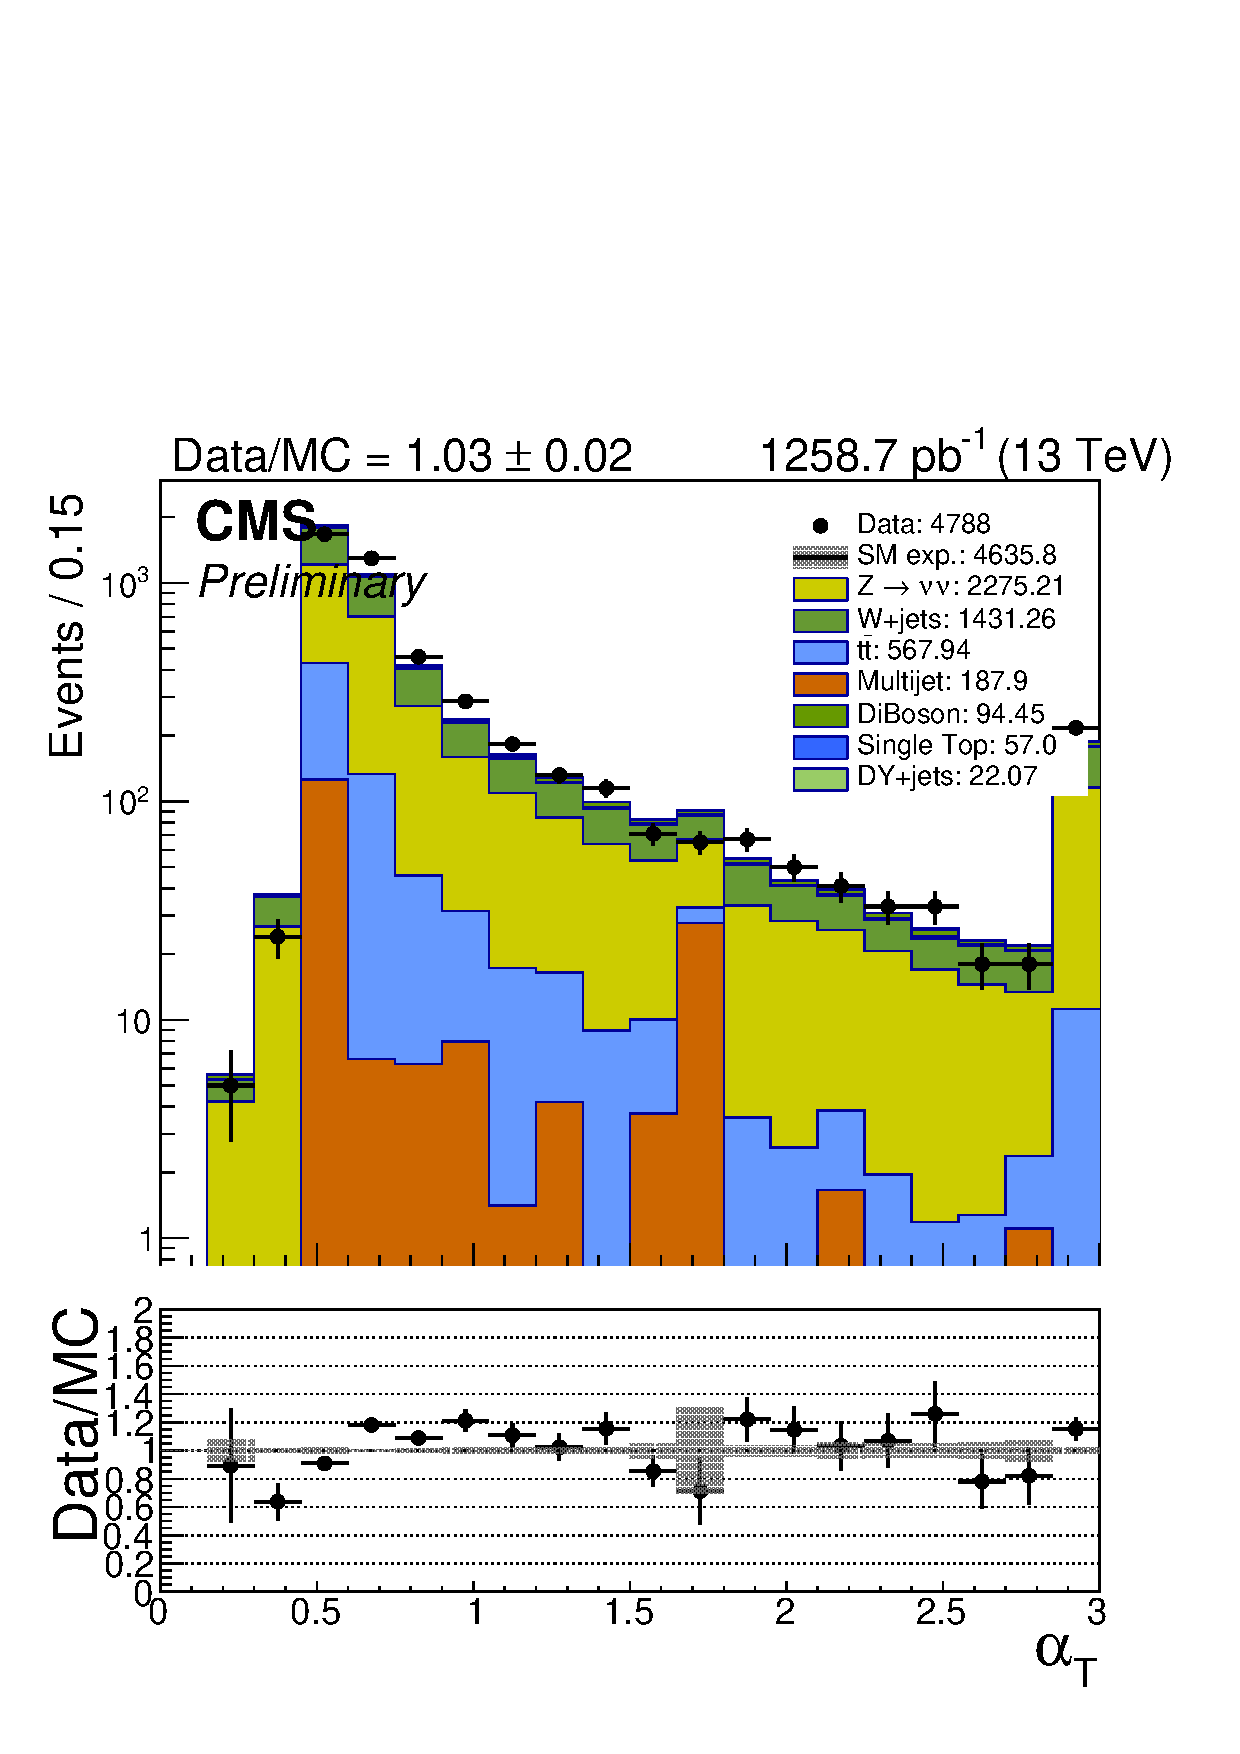
\includegraphics[width=0.5\textwidth]{figures/distributions/Signal/alphaT_sym.pdf}} ~~
        \subfigure {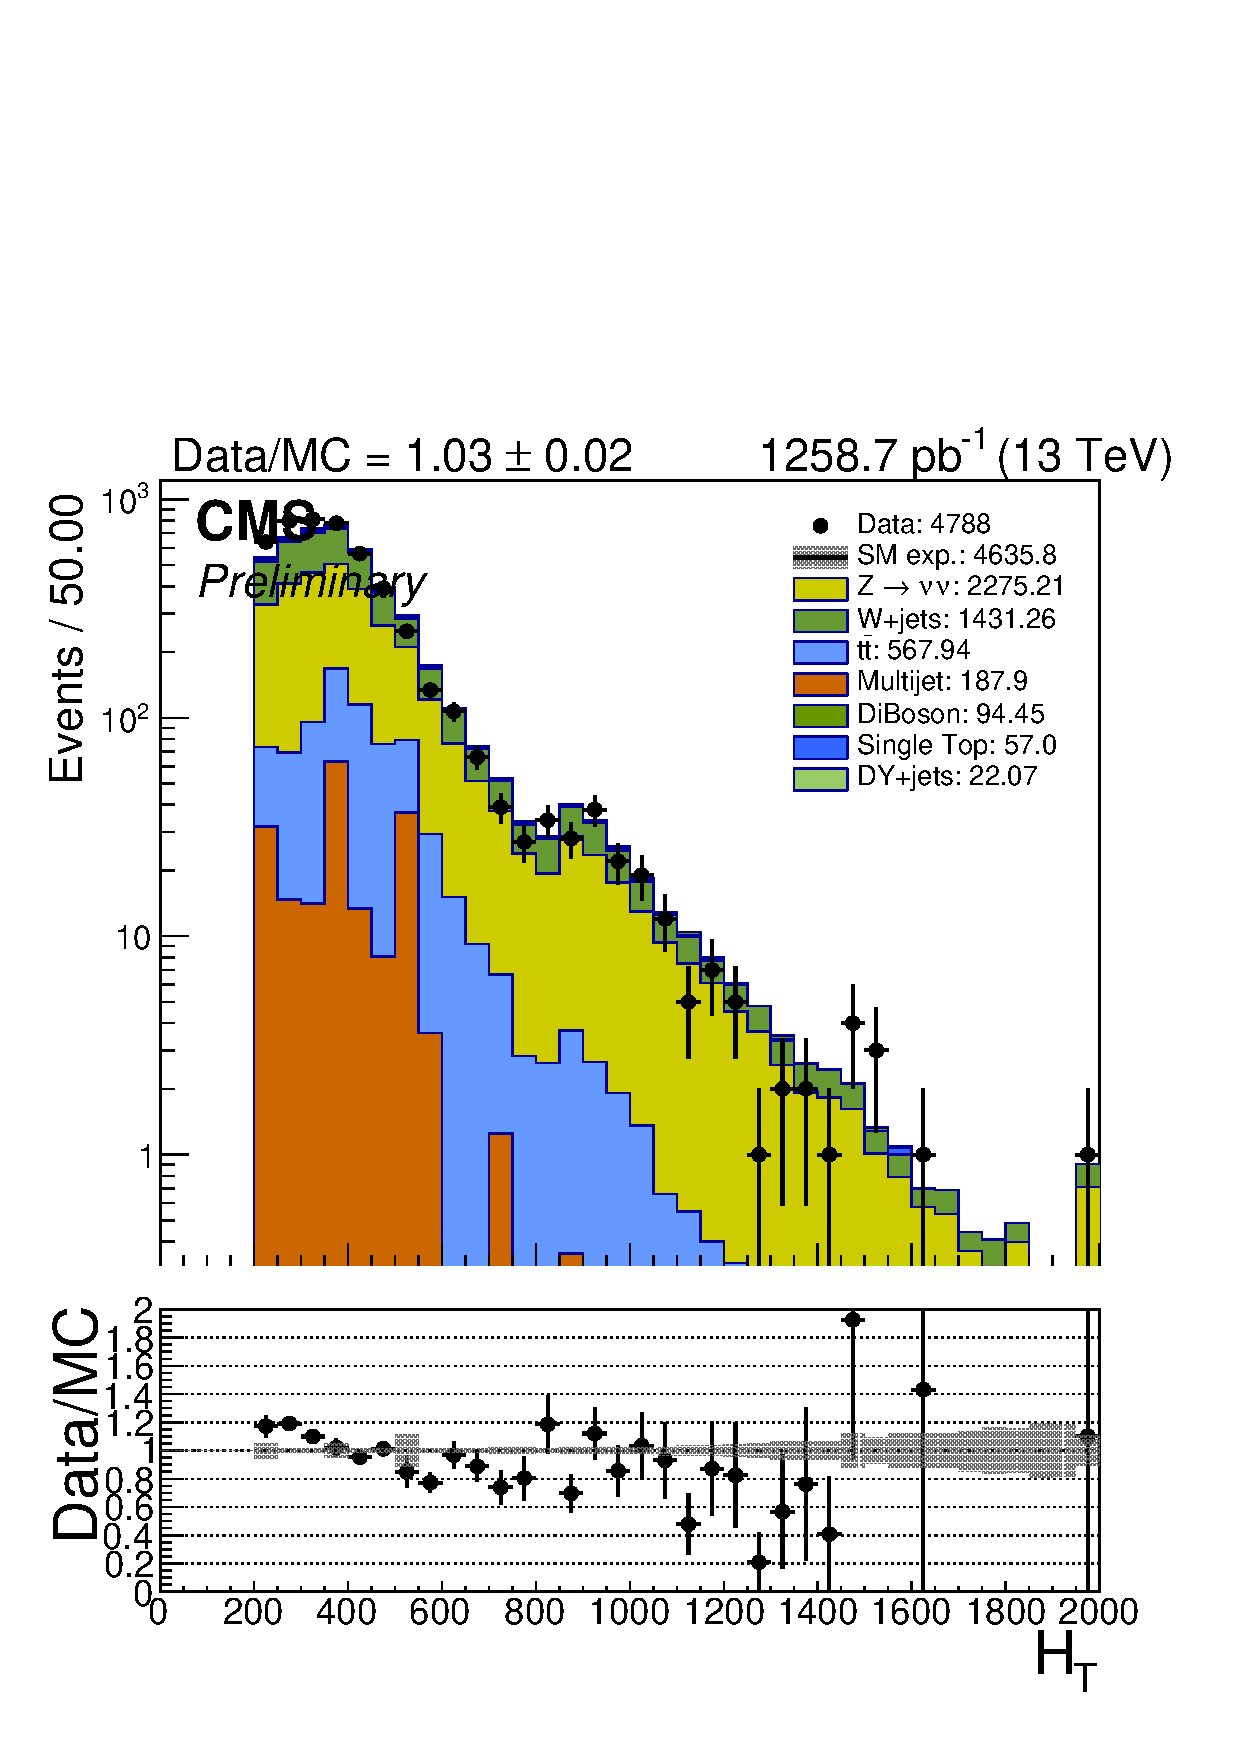
\includegraphics[width=0.5\textwidth]{figures/distributions/Signal/ht40_sym.pdf}} \\
        \subfigure {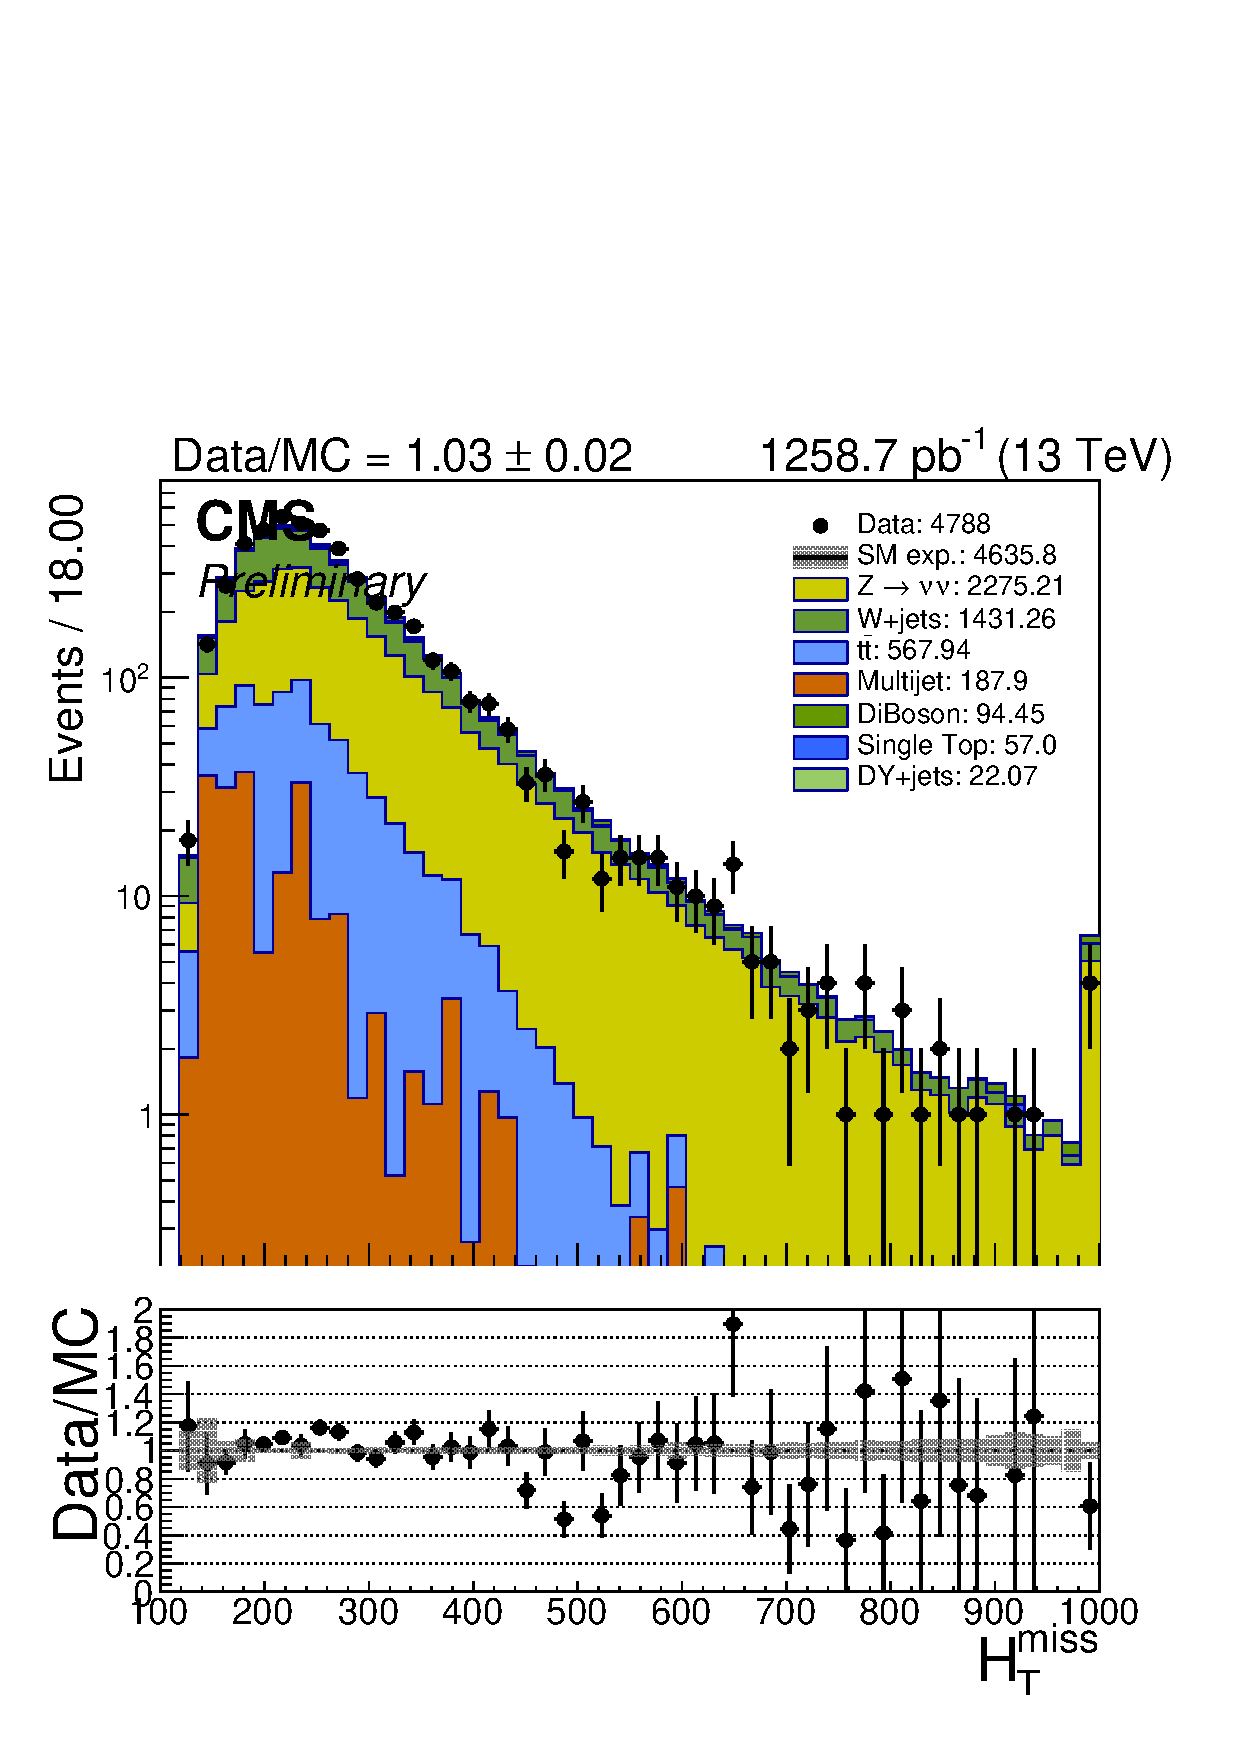
\includegraphics[width=0.5\textwidth]{figures/distributions/Signal/mht40_pt_sym.pdf}} ~~
        \subfigure {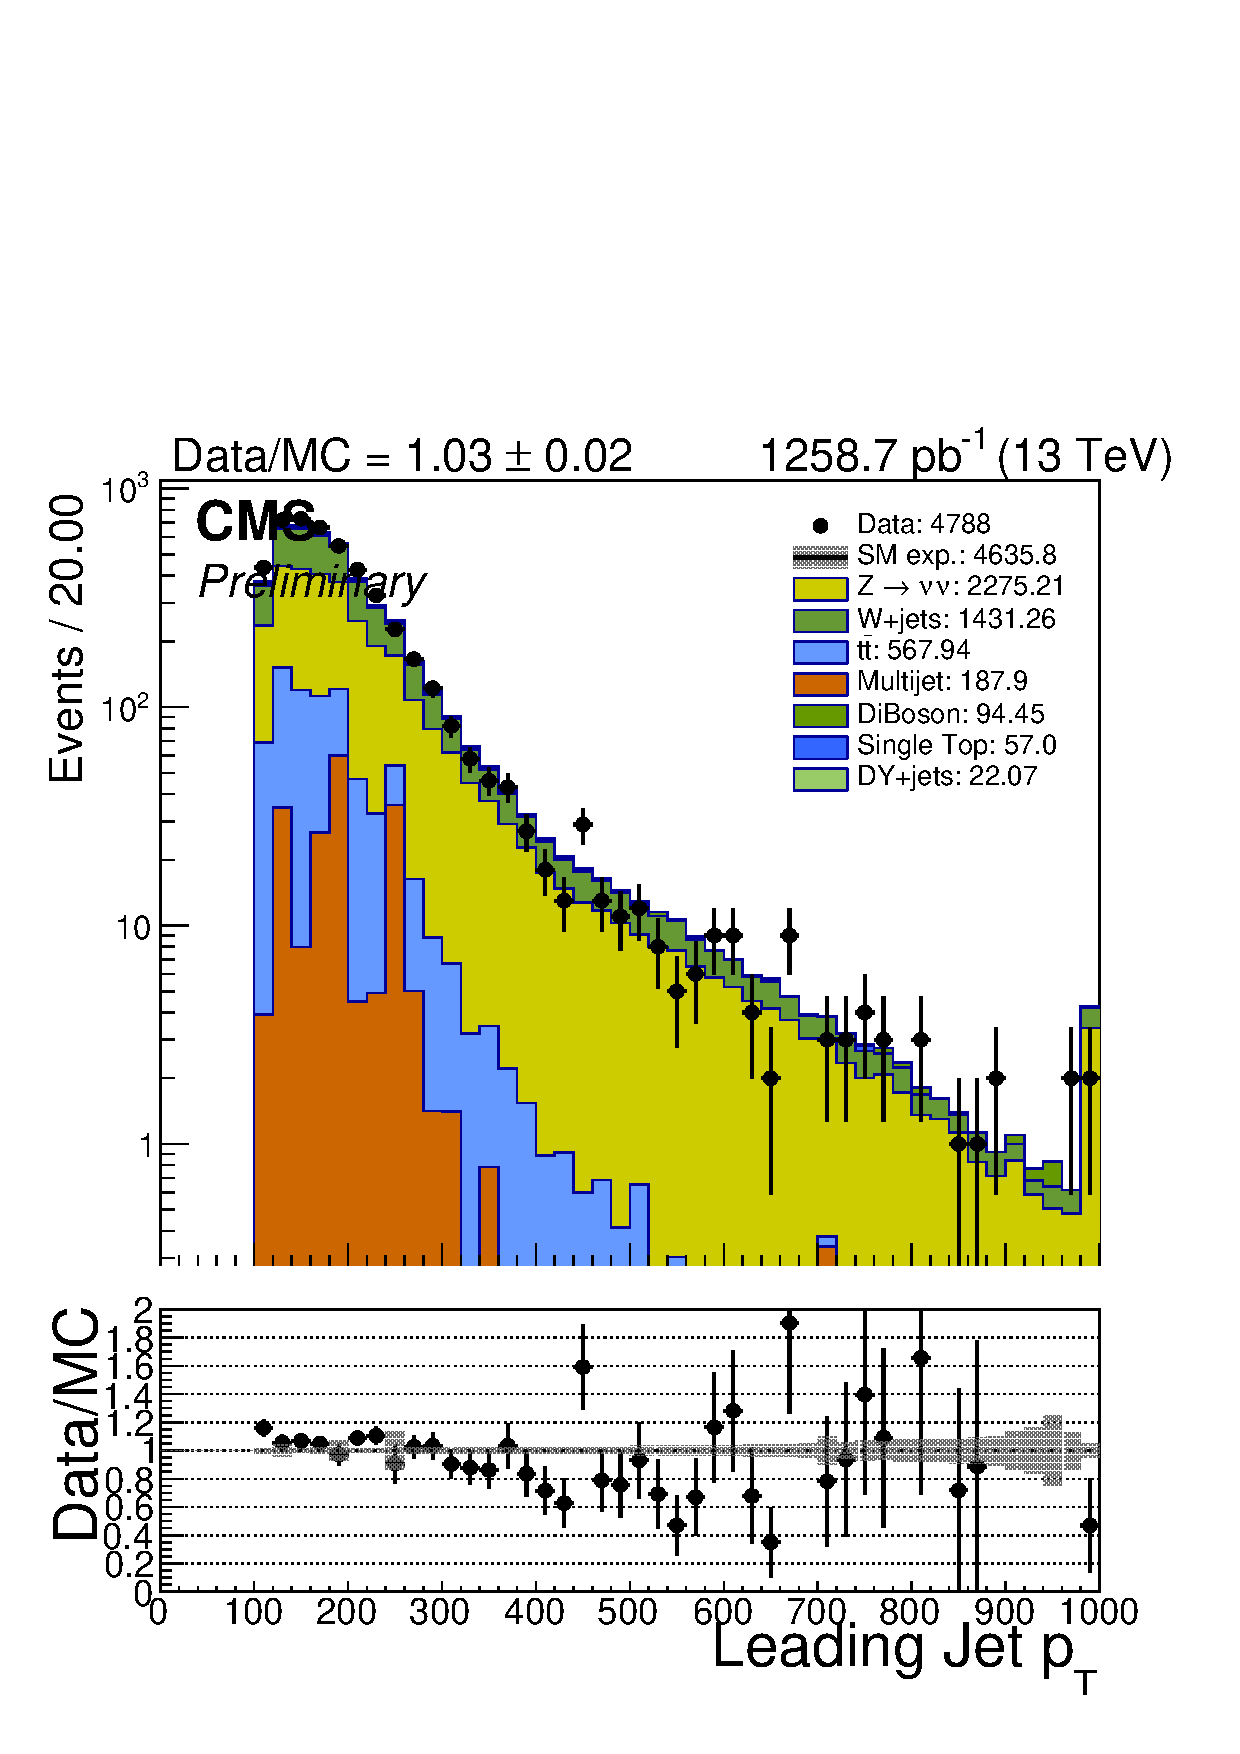
\includegraphics[width=0.5\textwidth]{figures/distributions/Signal/jet_pt[0]_sym.pdf}} \\
        \caption{Key analysis variables for hadronic signal region (symmetric \njet bins)}
        \label{fig:distribution_signal_sym}
    \end{center}
\end{figure}

\clearpage
\begin{figure}
    \begin{center}
        \subfigure {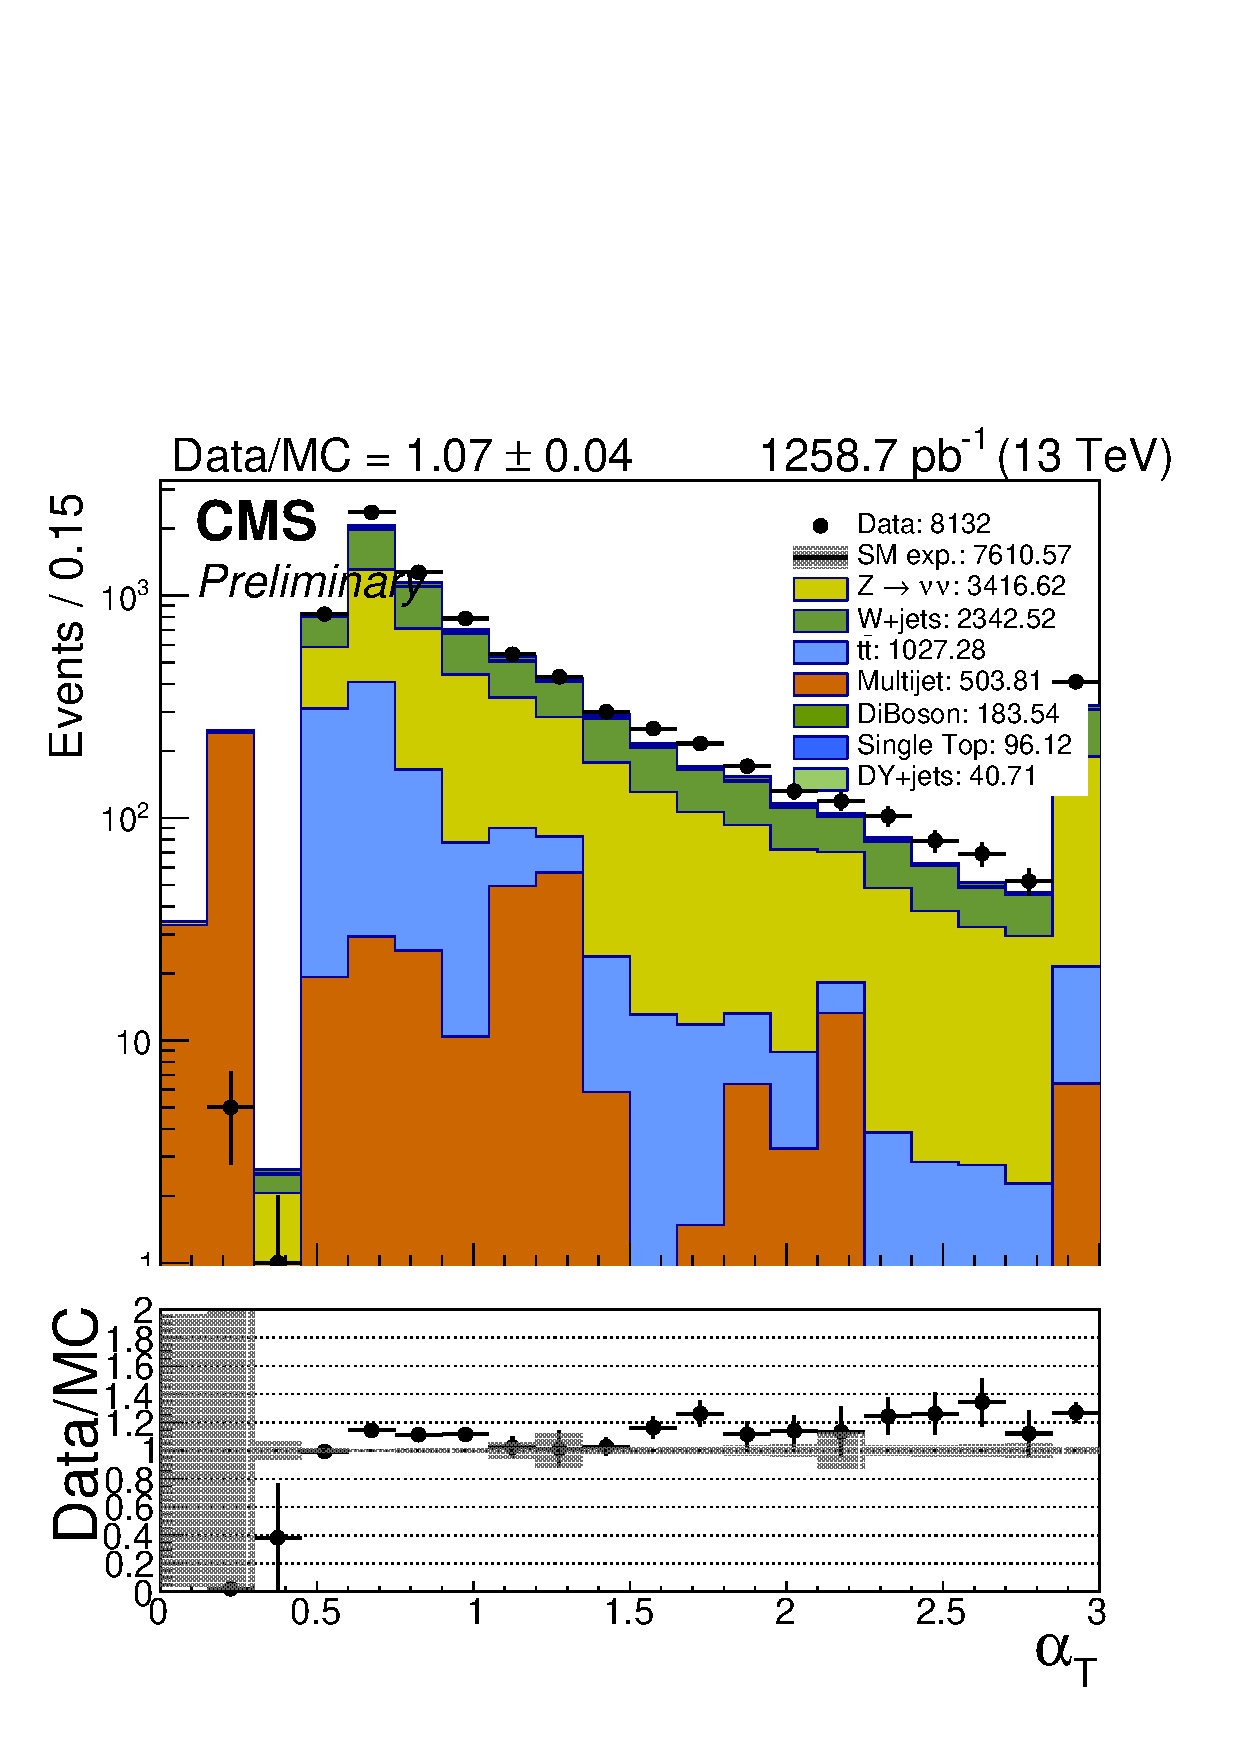
\includegraphics[width=0.5\textwidth]{figures/distributions/Signal/alphaT_asym.pdf}} ~~
        \subfigure {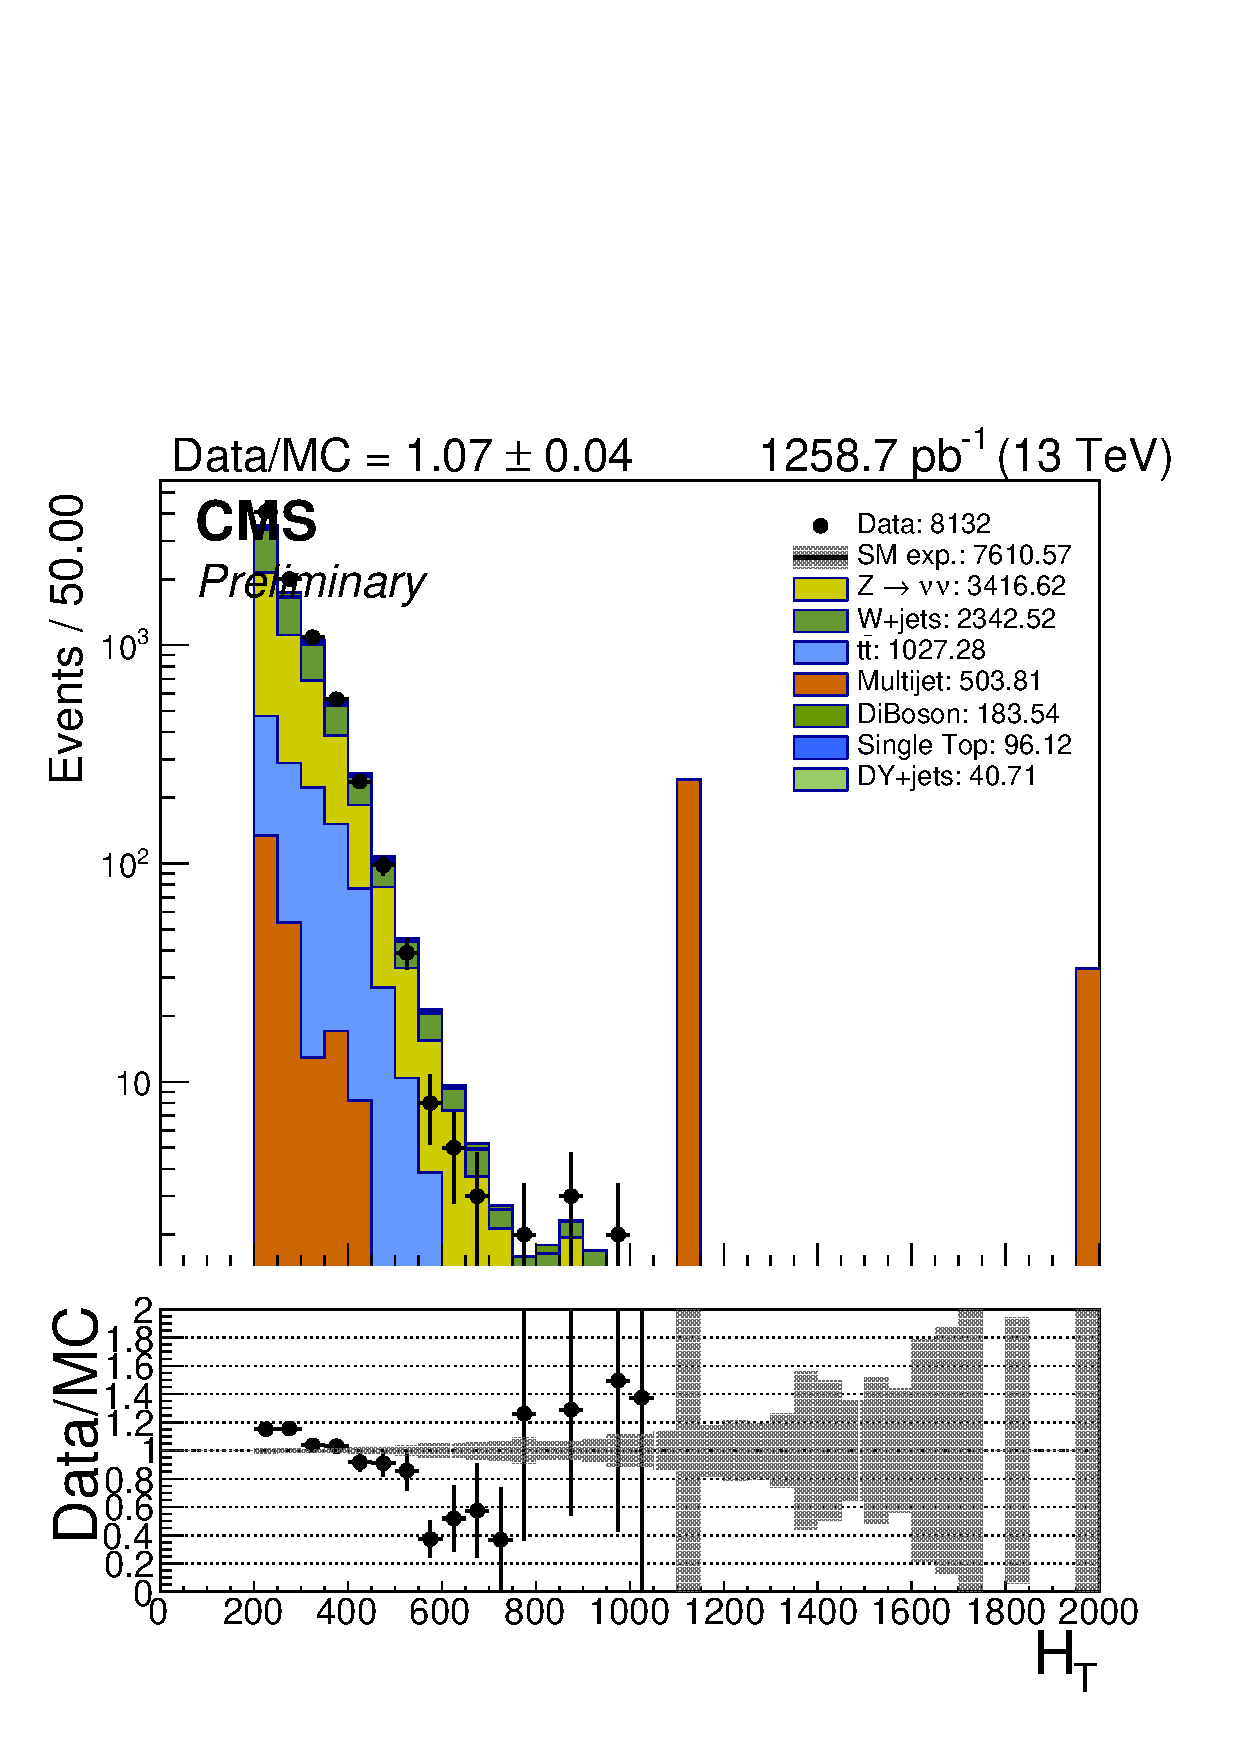
\includegraphics[width=0.5\textwidth]{figures/distributions/Signal/ht40_asym.pdf}} \\
        \subfigure {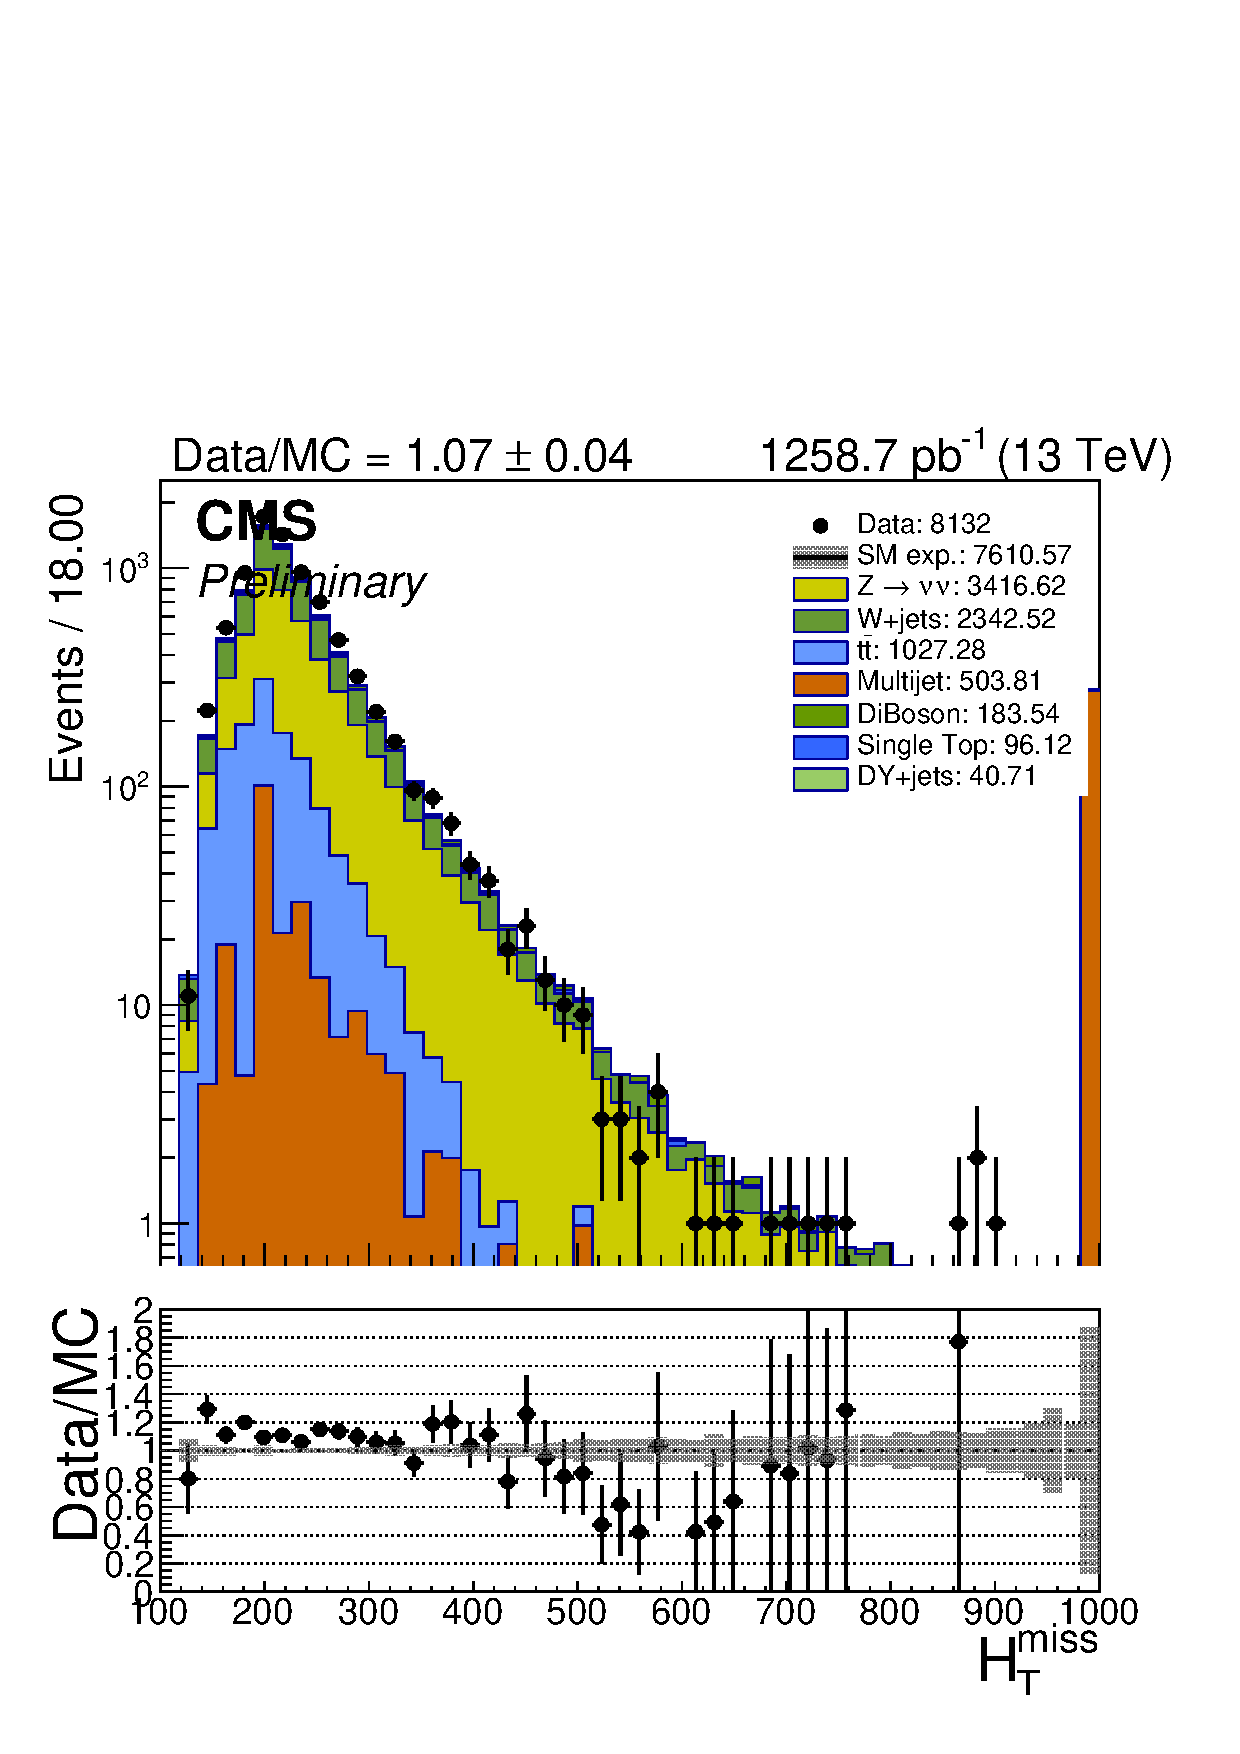
\includegraphics[width=0.5\textwidth]{figures/distributions/Signal/mht40_pt_asym.pdf}} ~~
        \subfigure {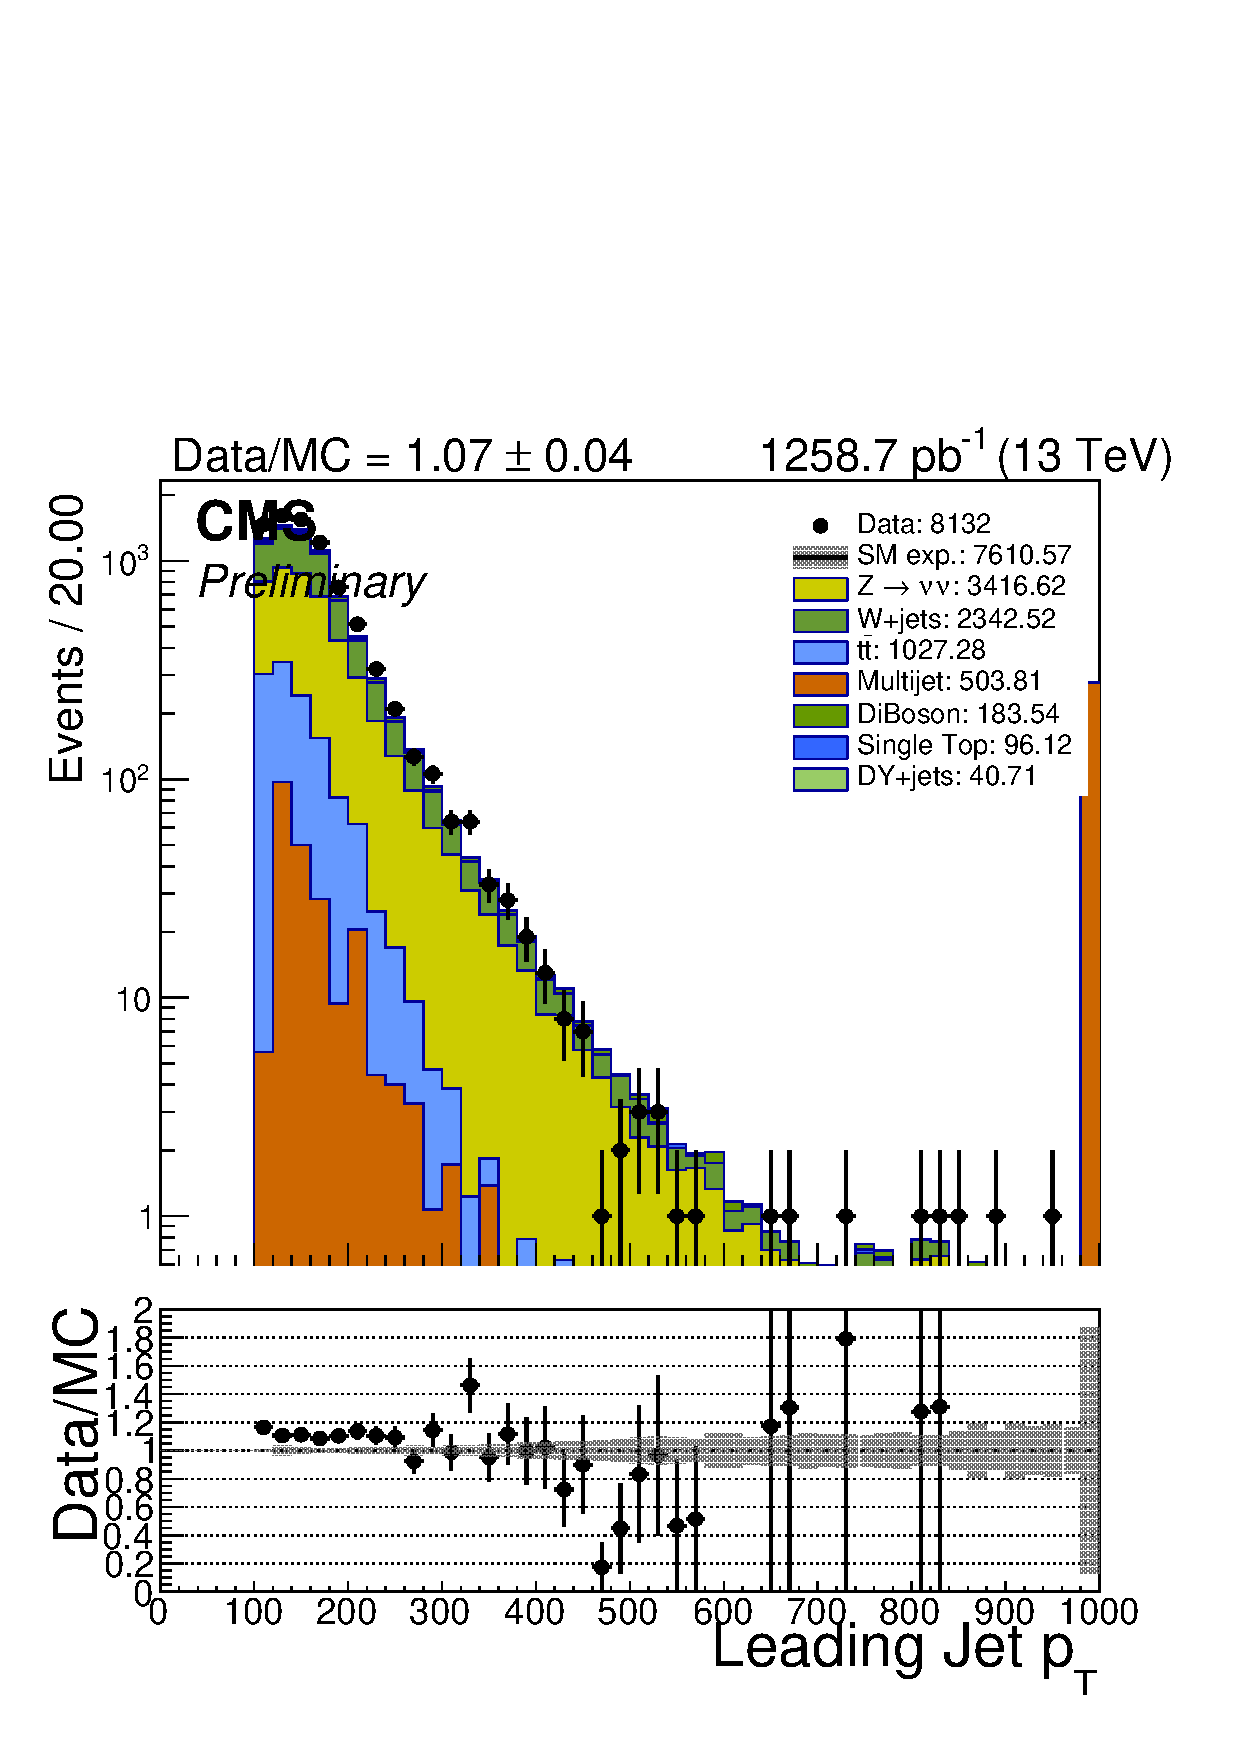
\includegraphics[width=0.5\textwidth]{figures/distributions/Signal/jet_pt[0]_asym.pdf}} \\
        \caption{Key analysis variables for hadronic signal region (asymmetric \njet bins)}
        \label{fig:distribution_signal_asym}
    \end{center}
\end{figure}

\clearpage
\begin{figure}
    \begin{center}
        \subfigure {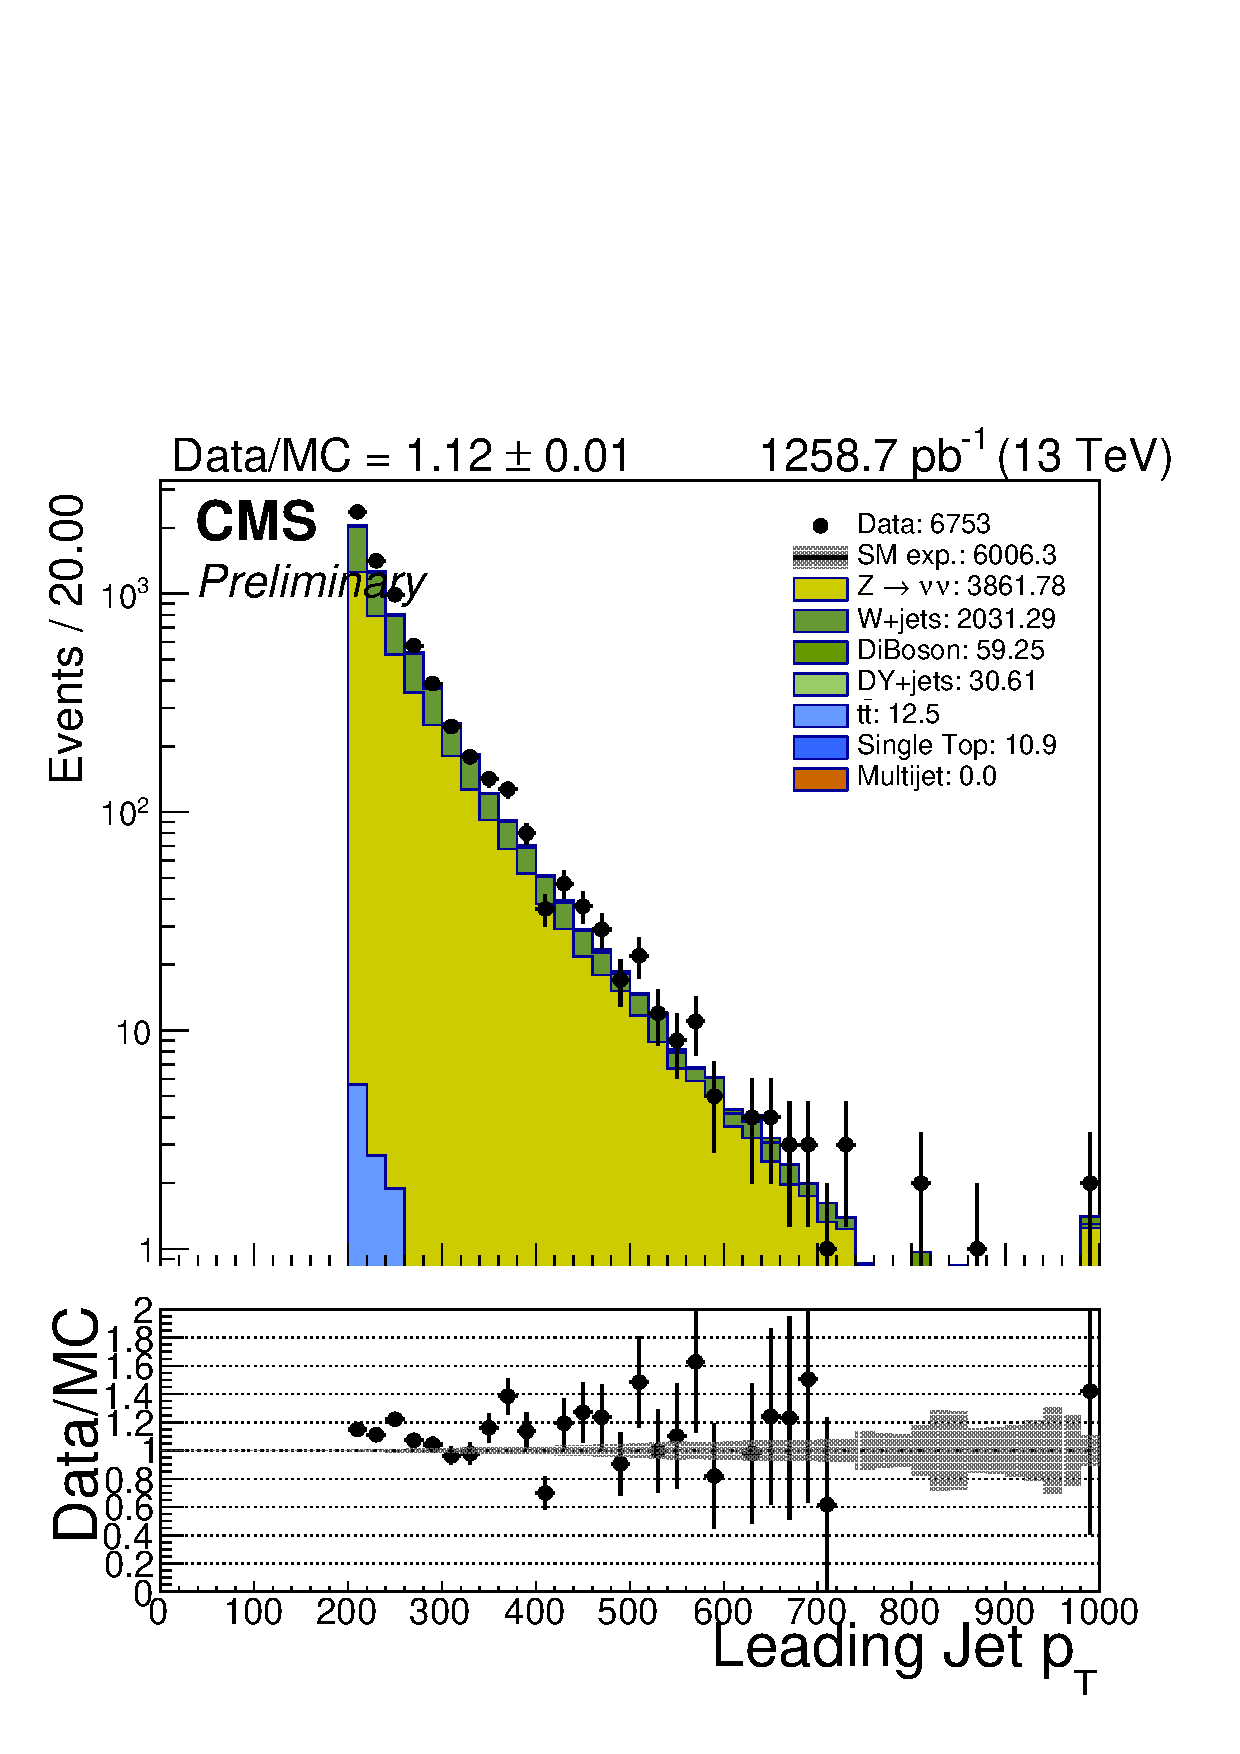
\includegraphics[width=0.5\textwidth]{figures/distributions/Signal/jet_pt[0]_eq1j.pdf}} ~~
        \subfigure {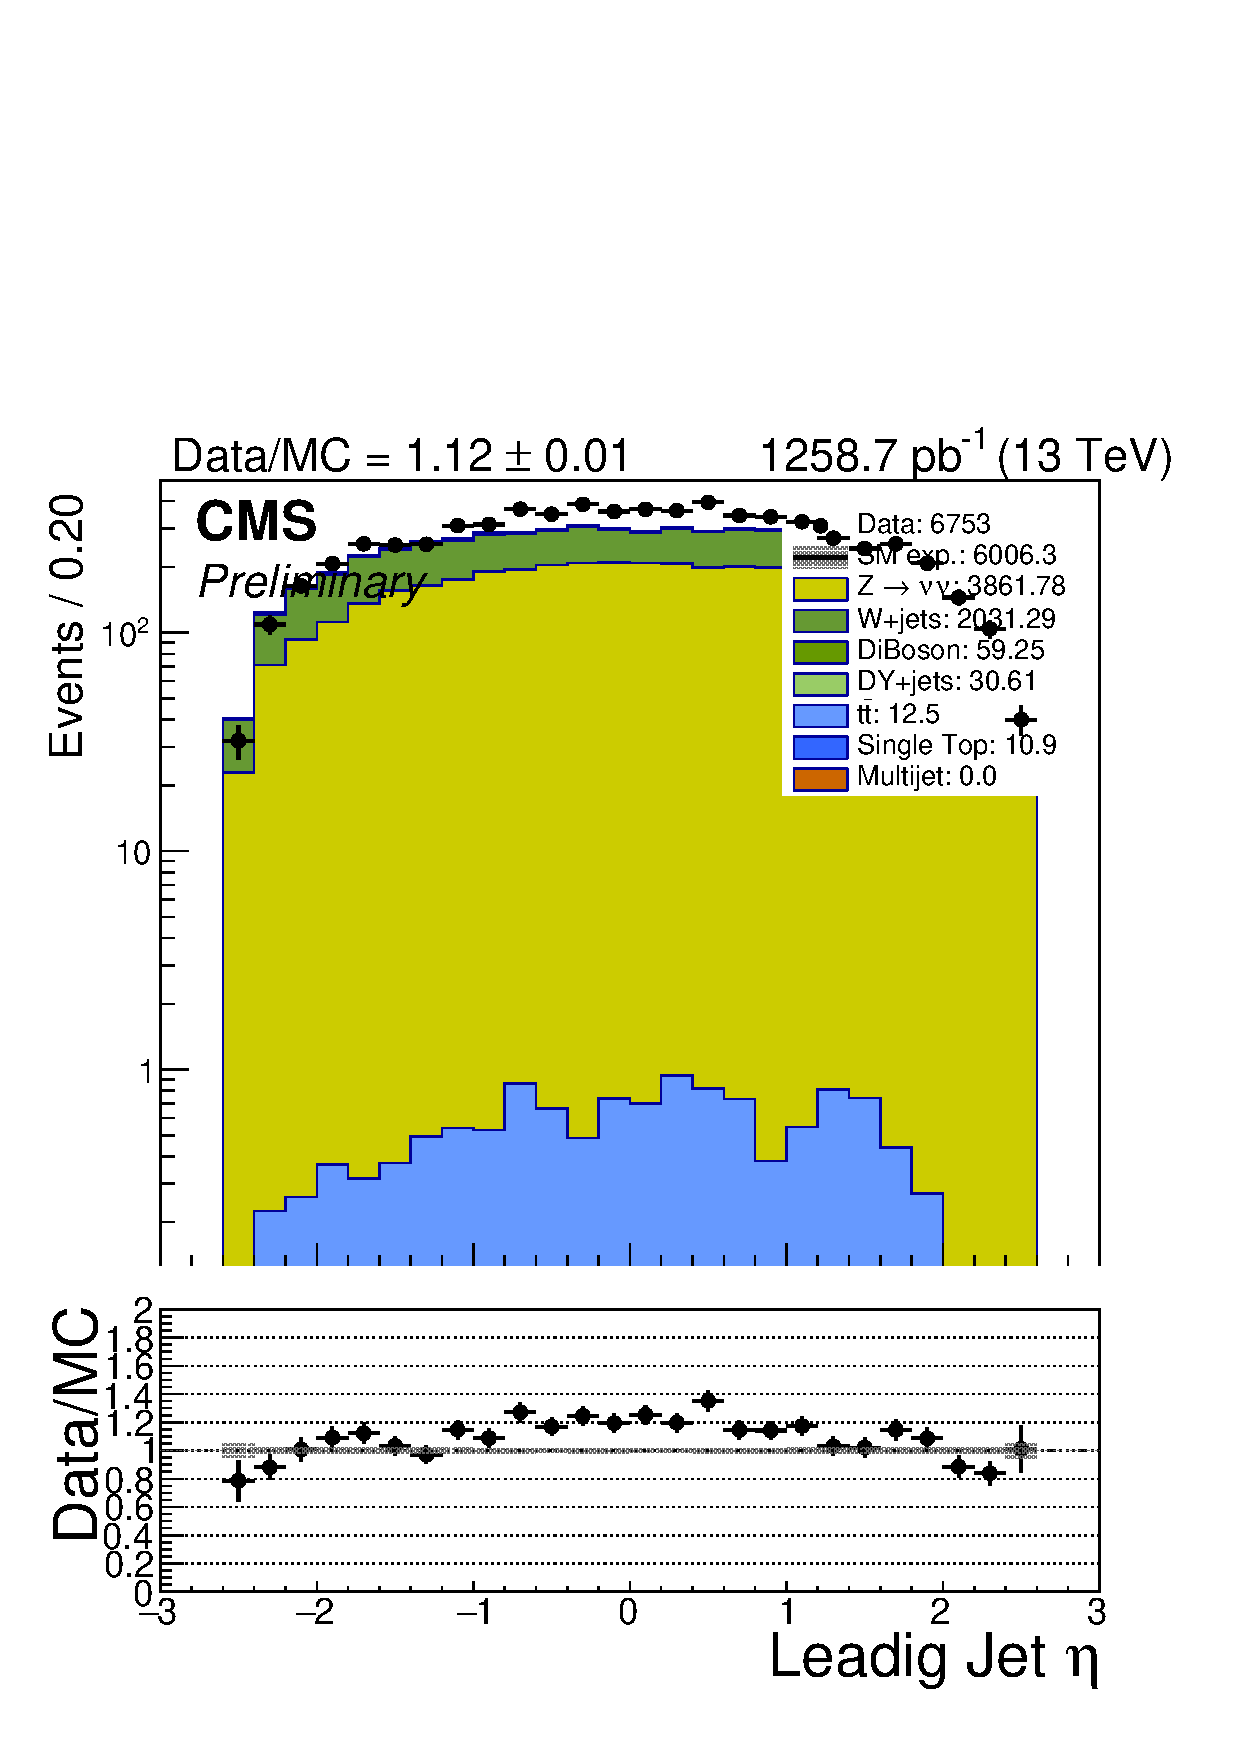
\includegraphics[width=0.5\textwidth]{figures/distributions/Signal/jet_eta[0]_eq1j.pdf}} \\
        \subfigure {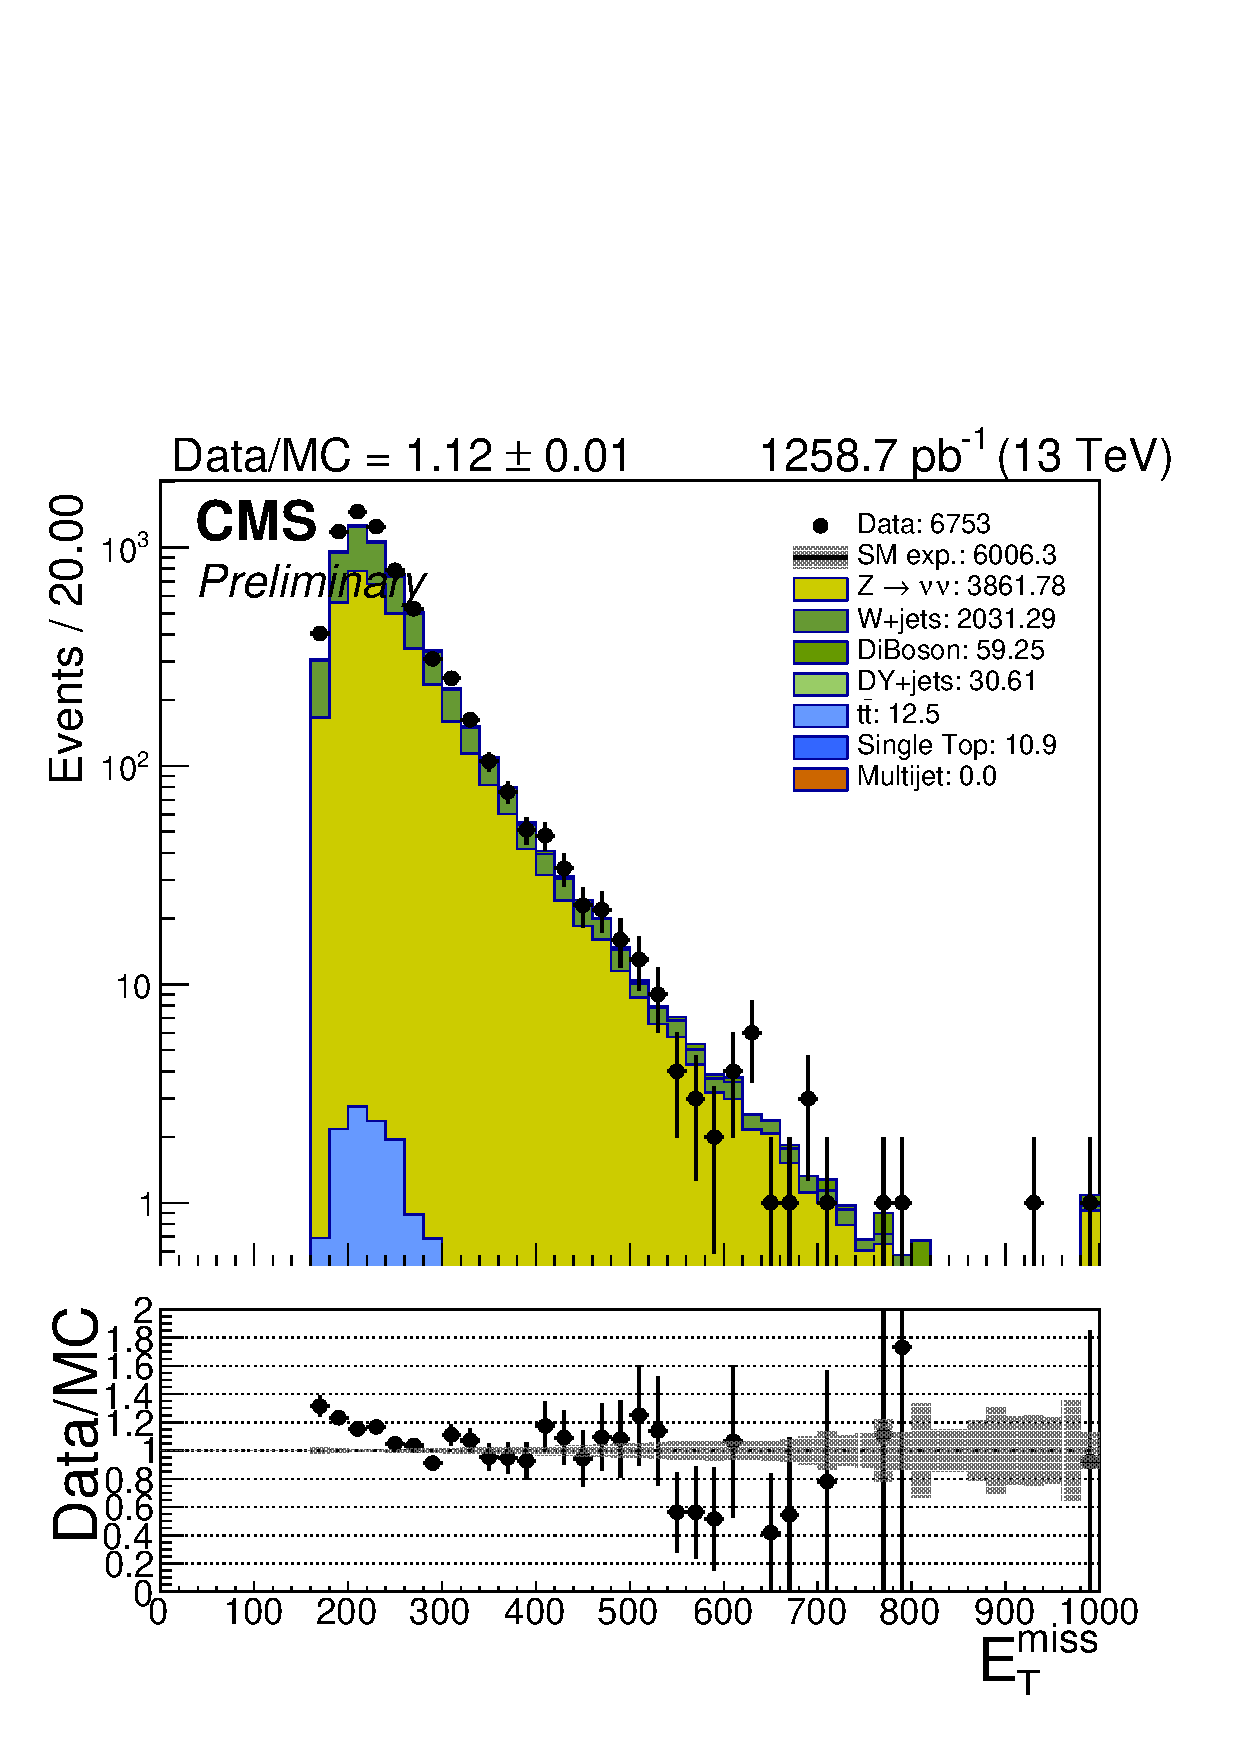
\includegraphics[width=0.5\textwidth]{figures/distributions/Signal/met_pt_eq1j.pdf}} ~~
        \subfigure {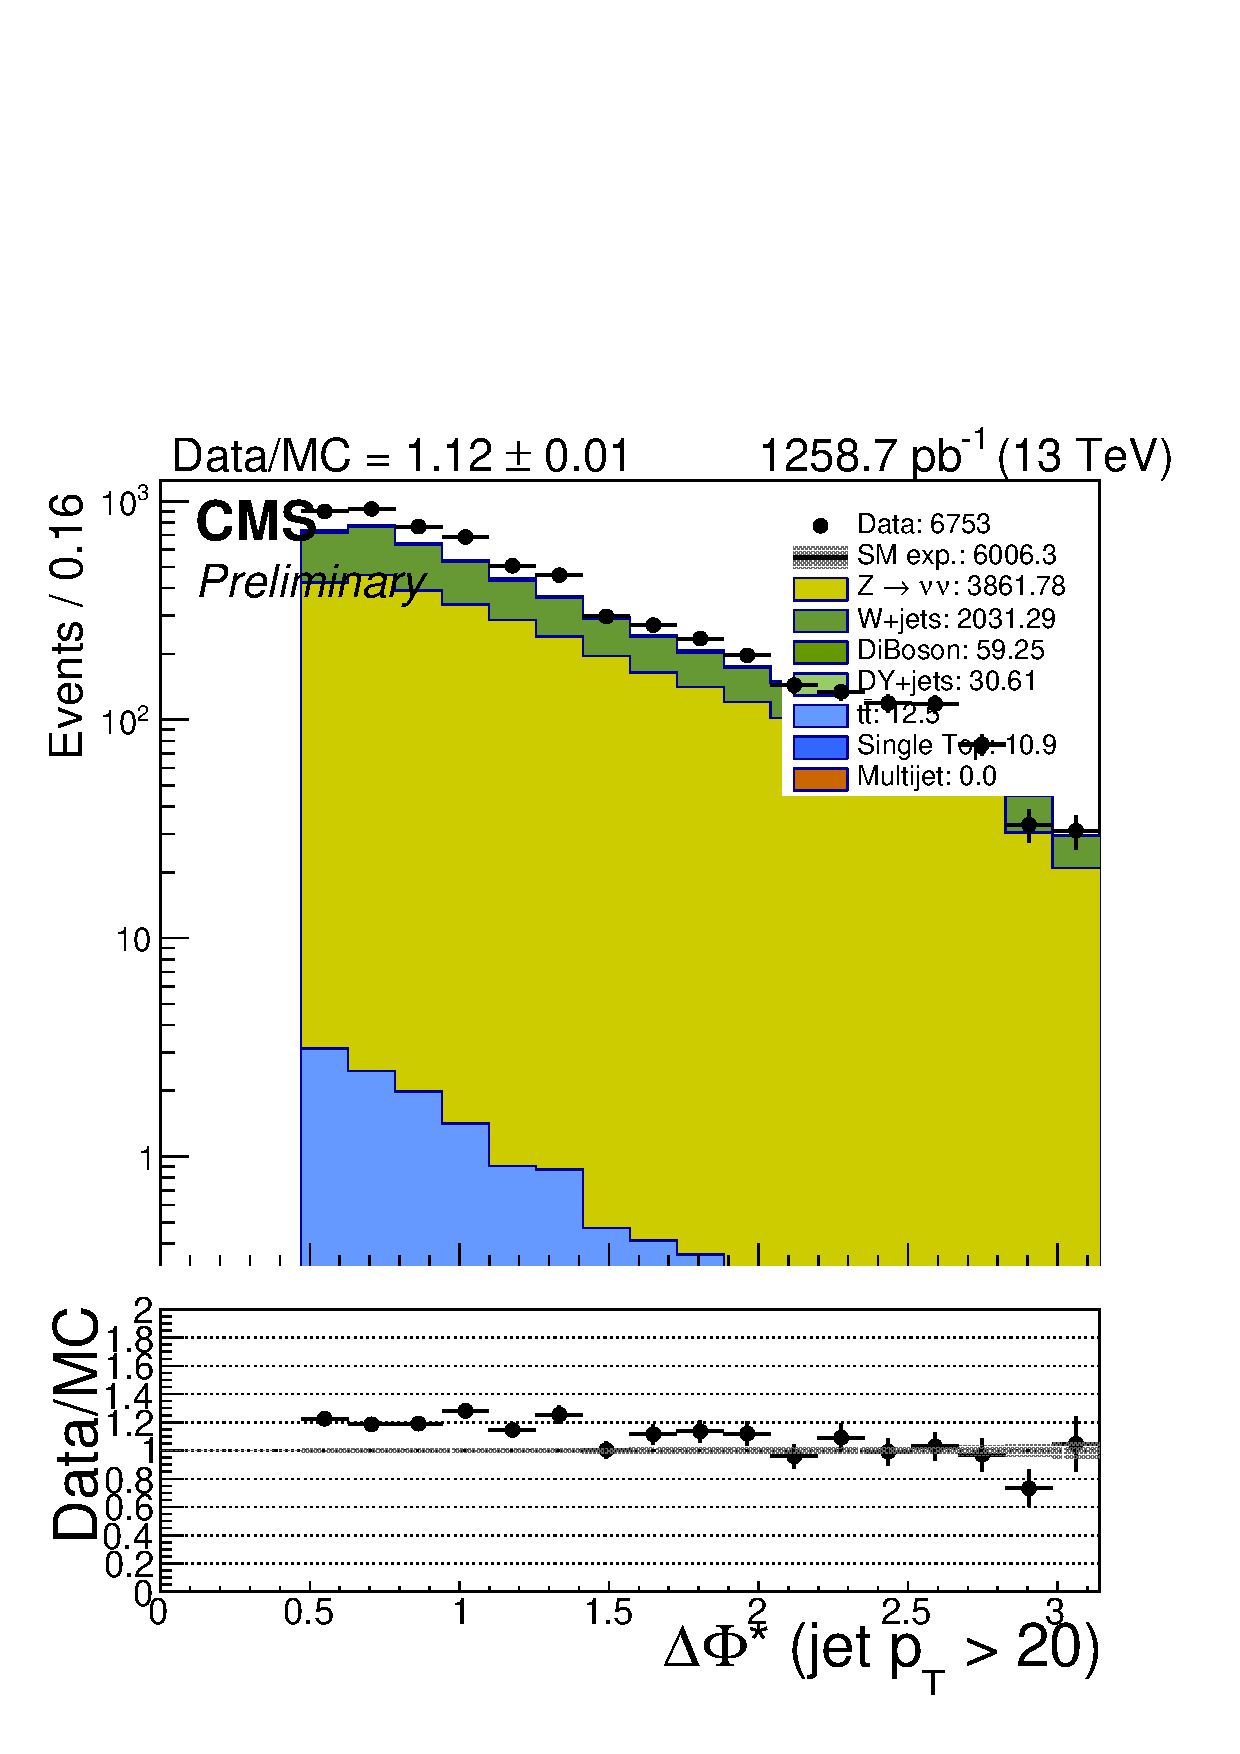
\includegraphics[width=0.5\textwidth]{figures/distributions/Signal/biasedDPhi20_eq1j.pdf}} \\
        \caption{Key analysis variables for hadronic signal region (monojet bins)}
        \label{fig:distribution_signal_mono}
    \end{center}
\end{figure}

